\documentclass[8pt]{beamer}
\usepackage[T1]{fontenc} 
\usepackage[francais]{babel}
\usepackage{tikz}
\usetikzlibrary{arrows,shapes}
\usepackage{pslatex}
\usepackage{textcomp}
\usepackage[utf8]{inputenc}  
\usepackage{picins}
\usepackage{wrapfig}
\usepackage{graphicx}
\usepackage[section]{placeins}
\usepackage{lscape}
\usepackage{float} 
\usepackage{amssymb}
\usepackage{wasysym}
\usepackage{pgf}
\usepackage{alltt}
\usepackage{eso-pic}
\usepackage{comment}
%\usepackage{enumitem}
\usepackage{ulem}

\usetheme{CambridgeUS}

\title[Arbor PFA]{ Arbor PFA \\ Update Separation of overlaid shower studies}
\institute[UCBL - IPNL]{Université Claude Bernard Lyon 1 - Institut de Physique Nucléaire de Lyon }
\author[R. Eté]{{\bf Eté Rémi}}
\date{\today}

\DeclareUnicodeCharacter{00A0}{ }

%\setlistdepth{9}

\setbeamertemplate{itemize items}[ball]
\definecolor{MyGreen}{rgb}{0.1,0.5,0.1}
\setbeamercolor{structure}{fg=red!70!black}
\setbeamercolor{block title}{bg=red!70!black,fg=black}
\addtobeamertemplate{block begin}{\pgfsetfillopacity{0.5}}{\pgfsetfillopacity{1}}
\setbeamertemplate{navigation symbols}{}
\setbeamertemplate{background canvas}{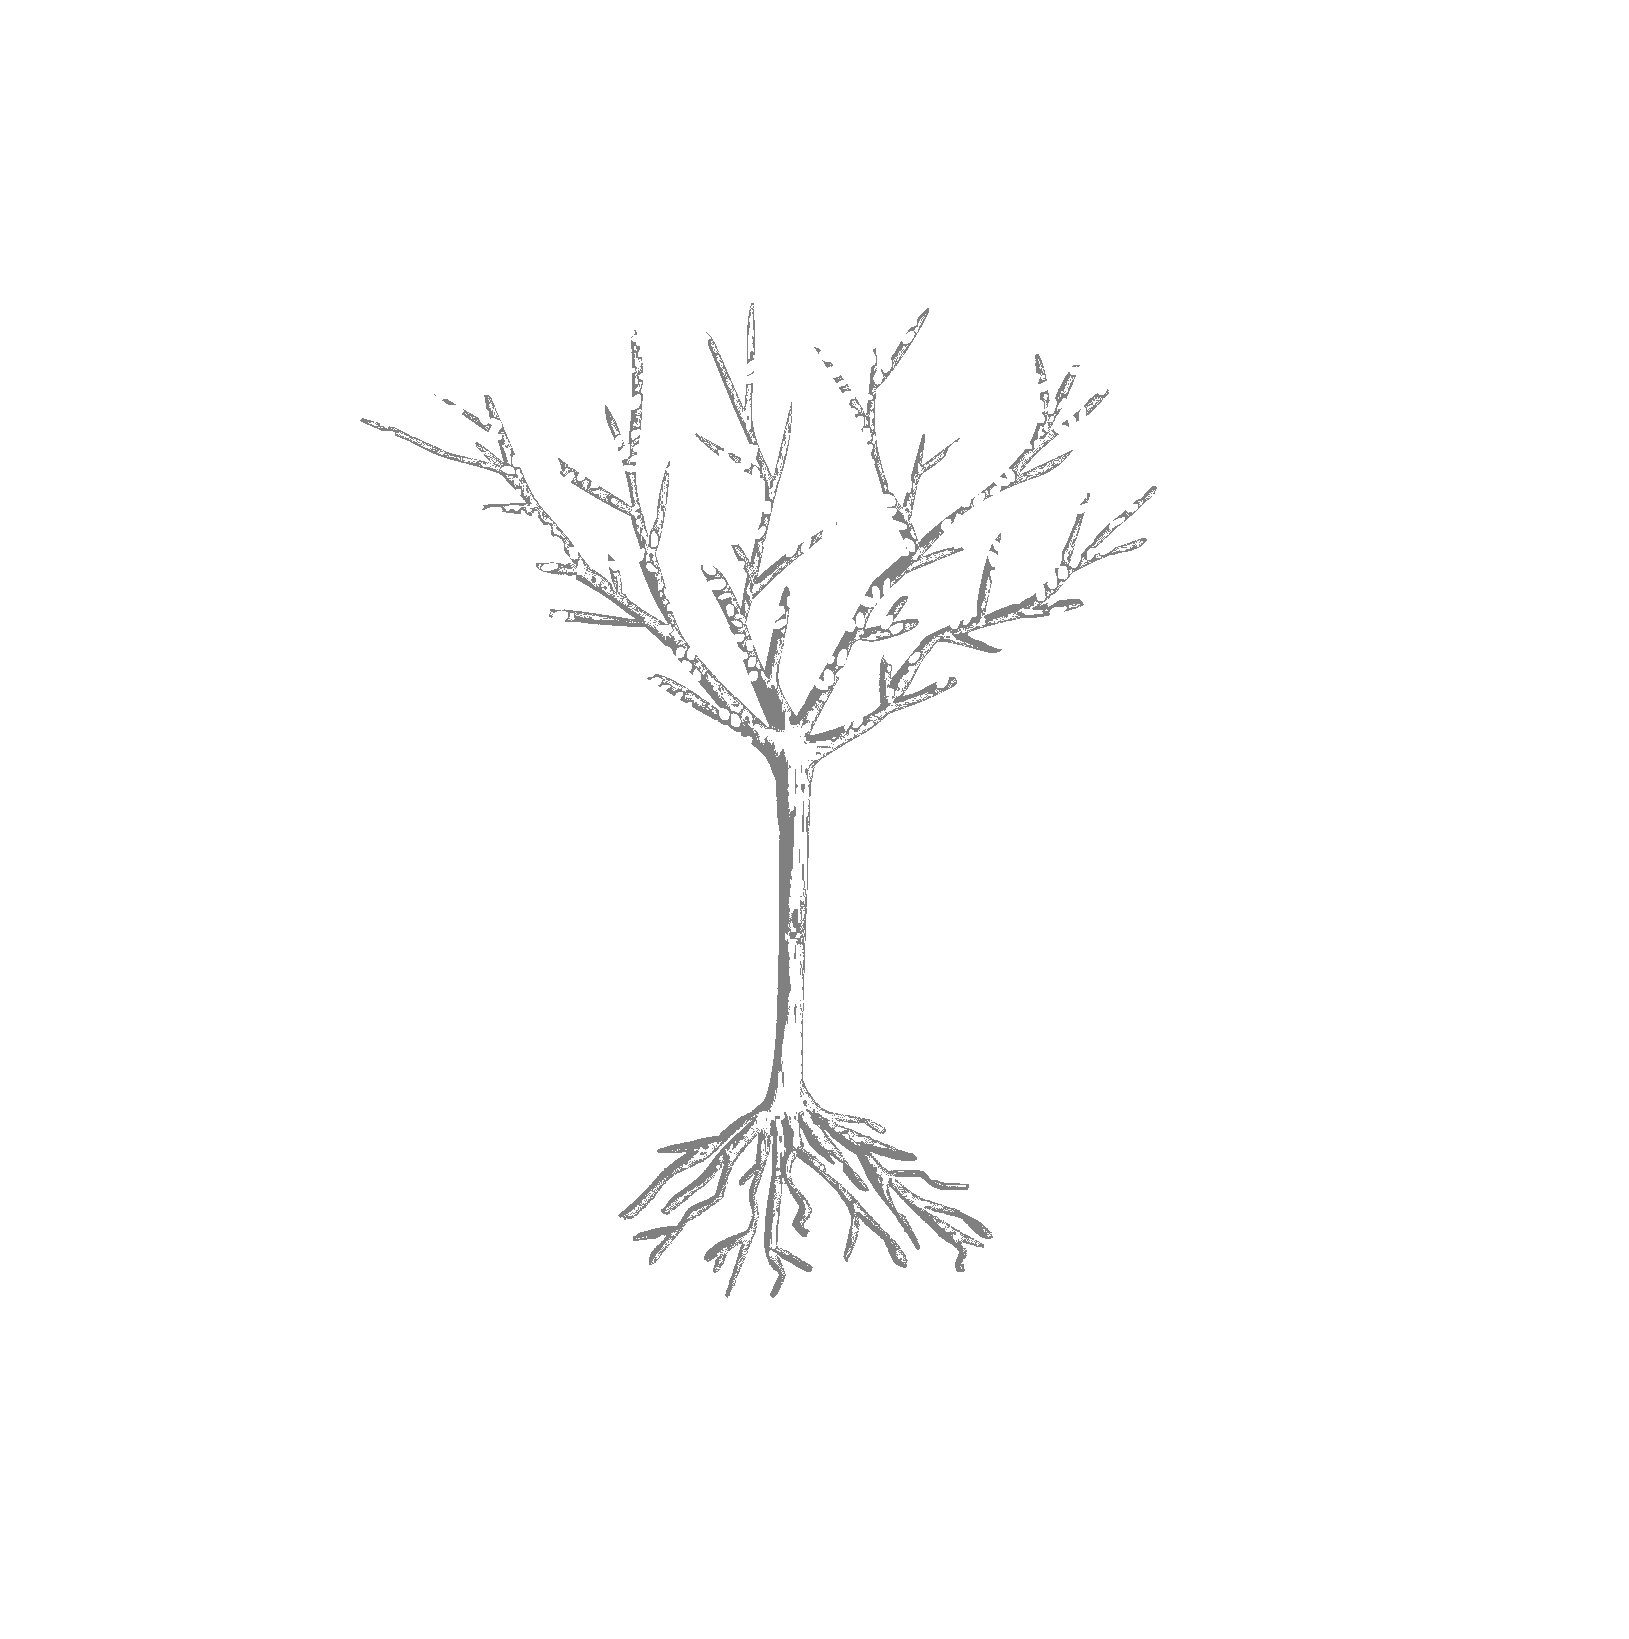
\includegraphics
   [width=\paperwidth,height=\paperheight]{img/arborLogo.jpg}}

\begin{document}

  %%%%%%%%%%%%%% Page de présentation %%%%%%%%%%%%%%
  \begin{frame}

    \titlepage
    \begin{center} 
      
\includegraphics[width=0.5\textwidth]{logo/logo-ucbl-ipnl.jpg} ~~~~~~~~~~~
      
\includegraphics[width=0.2\textwidth]{logo/logo_calice.png}
    \end{center}
  \end{frame}

  
  \setbeamertemplate{background canvas}{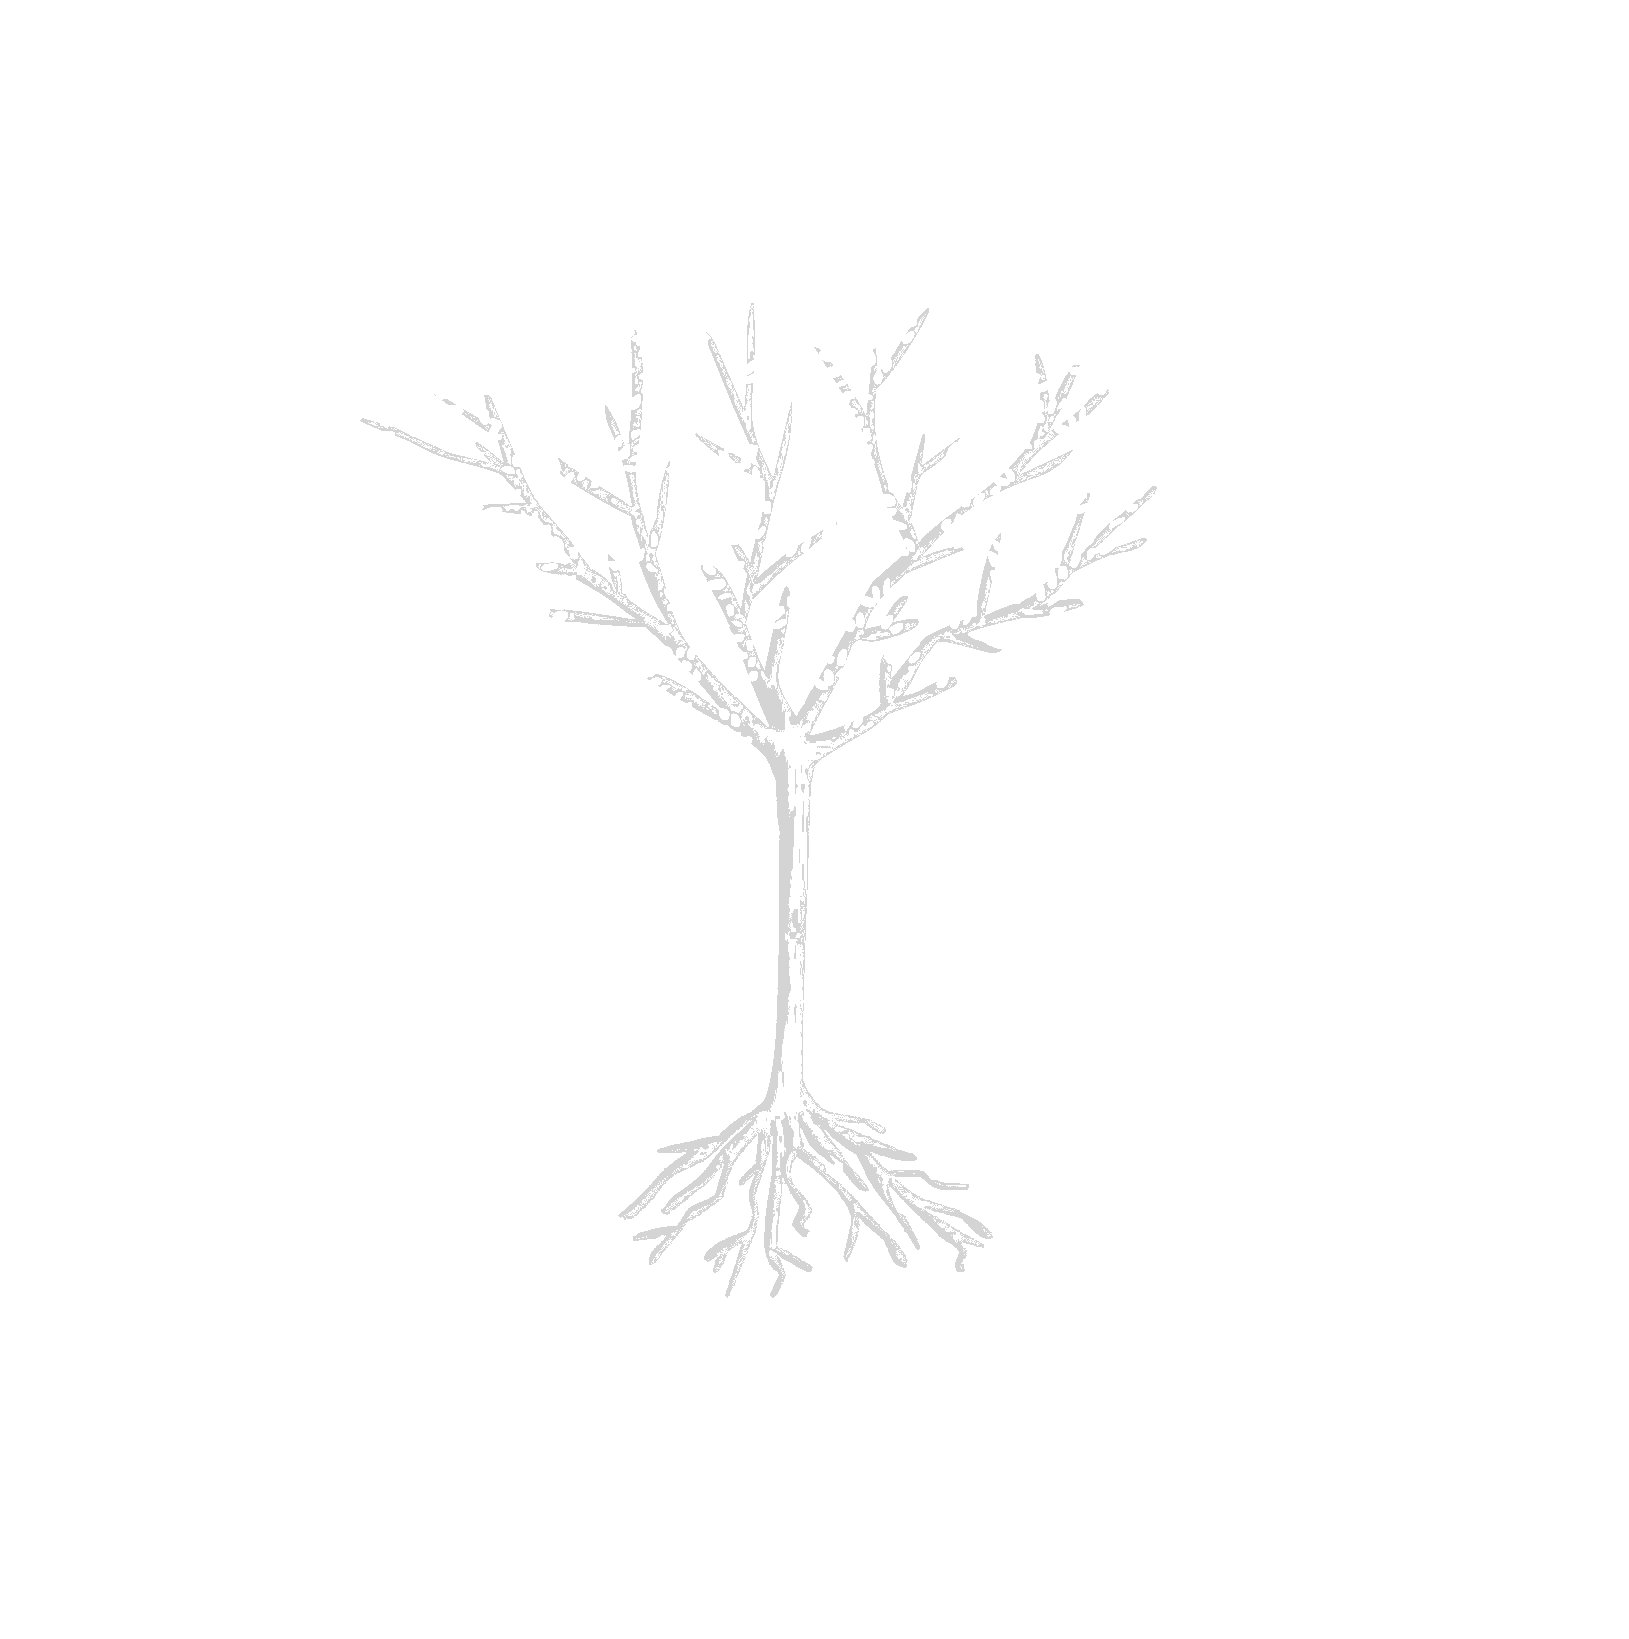
\includegraphics
   [width=\paperwidth,height=\paperheight]{img/arborLogoClair.jpg}}
   
  \begin{frame}
  \frametitle{Summary}
    \tableofcontents
  \end{frame}
  
  \section{Package review}
  
  \begin{frame}
  \frametitle{\secname}
  \framesubtitle{Softward package}
  
  Package currently under refactorization. \\ 
  Current is ArborPFA package v01-04-00 available at https://github.com/SDHCAL/ArborPFA \\
  Package based on PandoraSDK framework. \\
  ~ \\
  Currently working with J. Marshall to make the PandoraSDK framework extensible for base objects : CaloHit, Clusters, Tracks, Pfo, Vertex and MCParticle (CaloHit -> ArborCaloHit) \\
  ~ \\
  The whole code while be refactorized in new packages : \\
  \begin{enumerate}
    \item ArborContent : Algorithm content (https://github.com/rete/ArborContent)
    \item MarlinArbor : Marlin interface to ArborPFA (https://github.com/rete/MarlinArbor)
  \end{enumerate}
  ~ \\
  Interface is (already the case) the same as MarlinPandora with the same inputs that Pandora asks. \\
  Current documentation is only Doxygen.
  
  \end{frame}
  
  \begin{frame}
  \frametitle{\secname}
  \framesubtitle{Arbor algorithms + updates}
  
  ArborPFA (https://github.com/SDHCAL/ArborPFA) release \textcolor{red}{v01-04-00} \\ \pause

    \begin{enumerate}
      \item Object Creation \pause
      \item \sout{Isolation Tagging}
      \item \textcolor{blue}{Mip track CandidateTagging}\pause
      \item Connector Clustering Algorithm\pause
      \begin{enumerate}
        \item Connector Iteration Algorithms\pause
        \begin{enumerate}
          \item \textcolor{blue}{Primary Track Finder (local seeding and cleaning)}\pause
          \item Connector Seeding 1\pause
          \item Connector Cleaning 1\pause
          \item Connector Seeding 2\pause
          \item Connector Cleaning 2\pause
        \end{enumerate}
        \item Tree Building\pause
        \item Association Algorithms\pause
        \begin{enumerate}
          \item \sout{Topological Track Association}
          \item \textcolor{blue}{Energy Driven Track Association} \textcolor{red}{[E]} \pause
          \item \textcolor{blue}{Pointing Cluster Association} \textcolor{red}{[E]} \pause
          \item Neutral Tree Merging\pause
          \item Small Neutral Merging\pause
        \end{enumerate}
      \end{enumerate}
      \item Pfo Creation \pause
    \end{enumerate}
    
    Parameters retuned to reduce connection distance ... \\
    $\rightarrow$ More pfo splitting \textcolor{red}{(-)} \\
    $\rightarrow$ Separation more powerful \textcolor{blue}{(+)} \\
    ... BUT !! additionnal cluster association offsets this pfo splitting (reassociation) \textcolor{blue}{(+)}
   
  \end{frame}
  
  

  
  
  \section{Analysis updates}

  \begin{frame}
  \frametitle{\secname}
  \framesubtitle{Overview}
    
    \begin{itemize}
      \item Using SDHCAL with quadratic energy estimator function
      \item Single particle
      \begin{itemize}
        \item Efficiency
        \item N$_{pfos}$
        \item E$_{rec}$
        \item E$_{resol}$
      \end{itemize}
      \item Overlay event : a fake 10 GeV neutral hadron (cutting the primary track of a $\pi^-$) overlaid with a charged $\pi^-$ from 10 up to 50 GeV by a separation distance from 30 cm up to 5 cm.
      \begin{itemize}
        \item \textcolor{red}{N$_{pfos}$}
        \item Neutral particle hit \textcolor{red}{efficiency}
        \item Neutral particle hit \textcolor{red}{purity}.
        \item \textcolor{red}{Mean E$_{rec}$} and \textcolor{red}{mean E$_{rec}$-E$_{meas}$} from two different distributions i) the whole neutral energy distribution, ii) neutral energy distribution when at least one neutral particle has been reconstructed
        \item Using the E$_{n,rec}$ distribution (E$_{n,rec}$-E$_{n,meas}$ distribution), studying the \textcolor{red}{event fraction} contained in E$_{rec}~\pm~1\sigma_{E}$ (resp. $0~\pm1\sigma_{E}$)
        \item Same variables with $2\sigma_{E}$
      \end{itemize}

      \item No longer use PandoraPFA for comparison in this study. Too weird output results shown at HCG4ILD for TPC+SDHCAL only system (ConeClusteringAlgorithm not adapted).
    \end{itemize}

    
    
  \end{frame}

  \begin{frame}
  \frametitle{\secname}
  \framesubtitle{Single particle}
    \begin{center}
      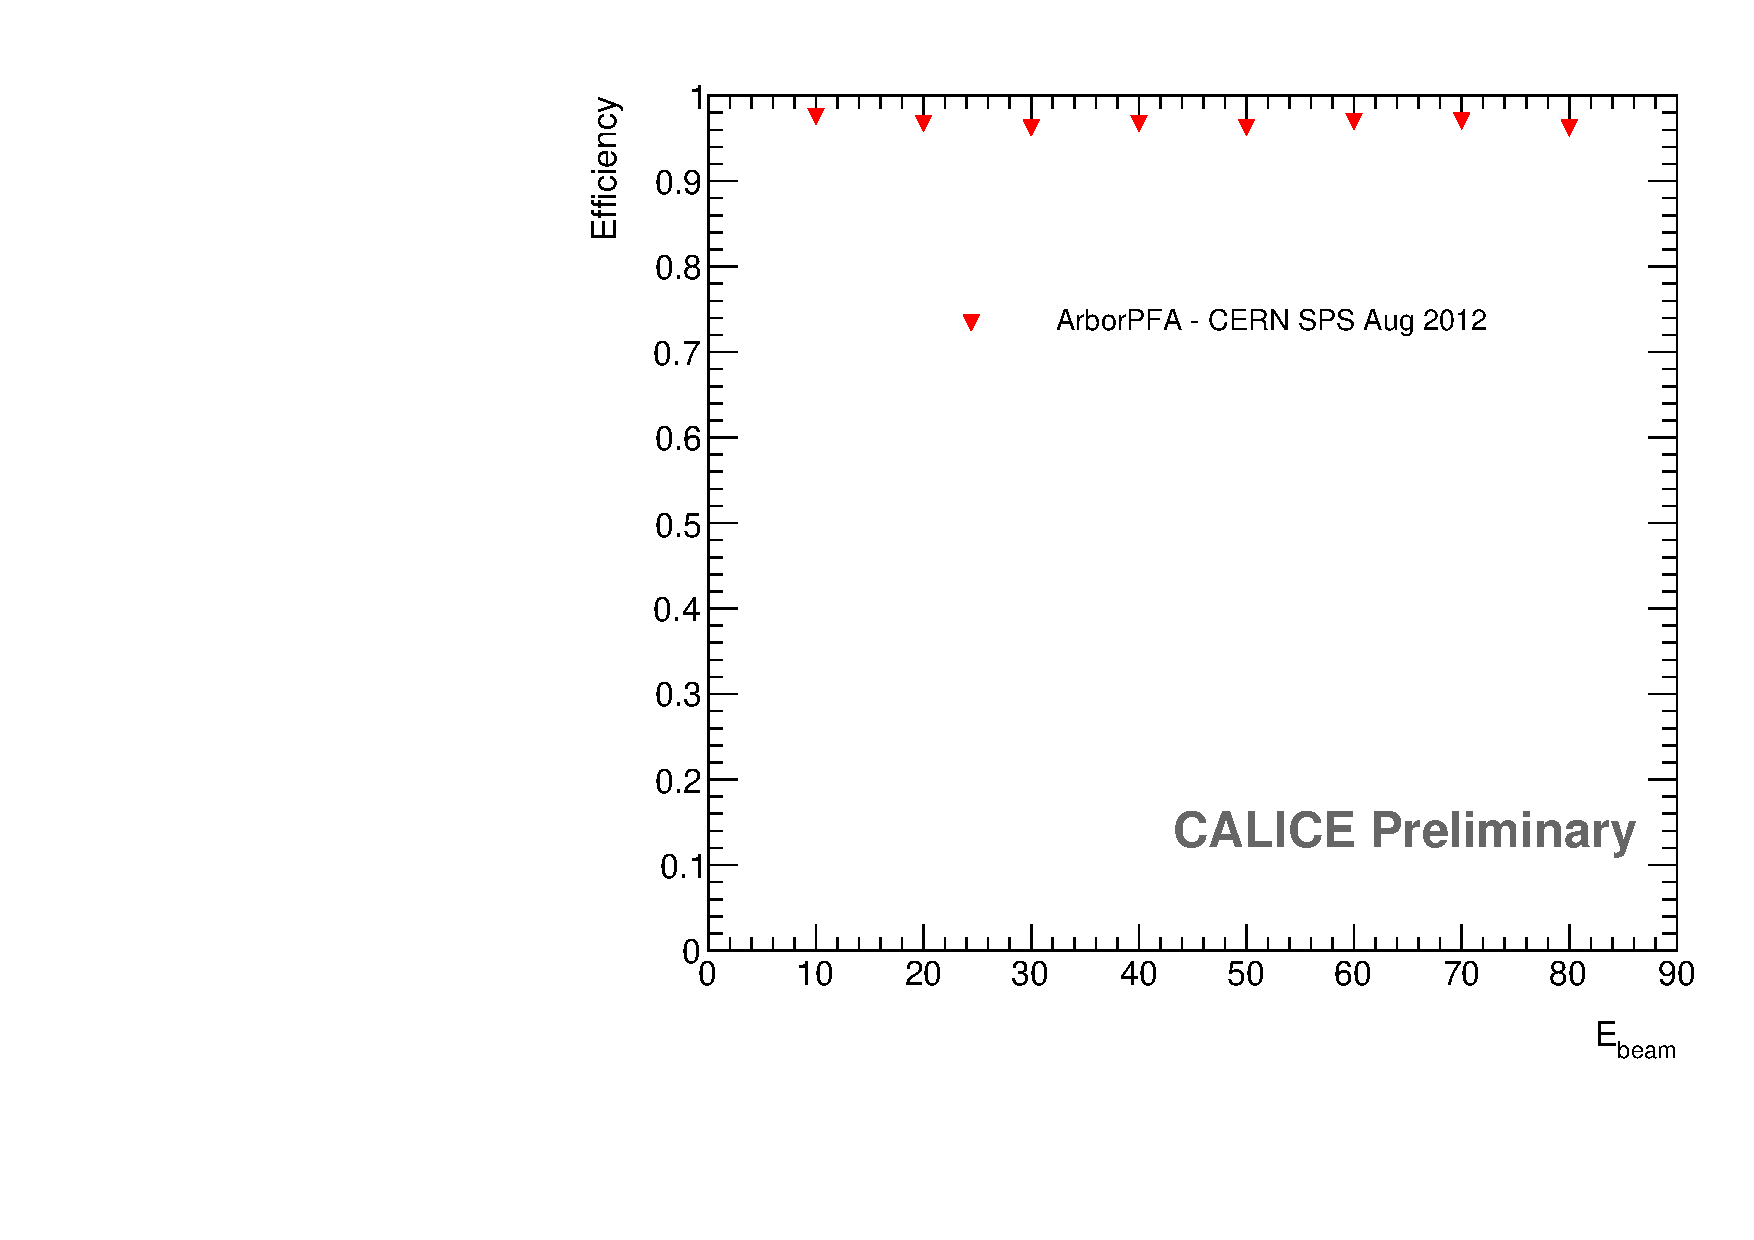
\includegraphics[width=0.5\textwidth]{plots/SingleParticle_Efficiency.pdf}
      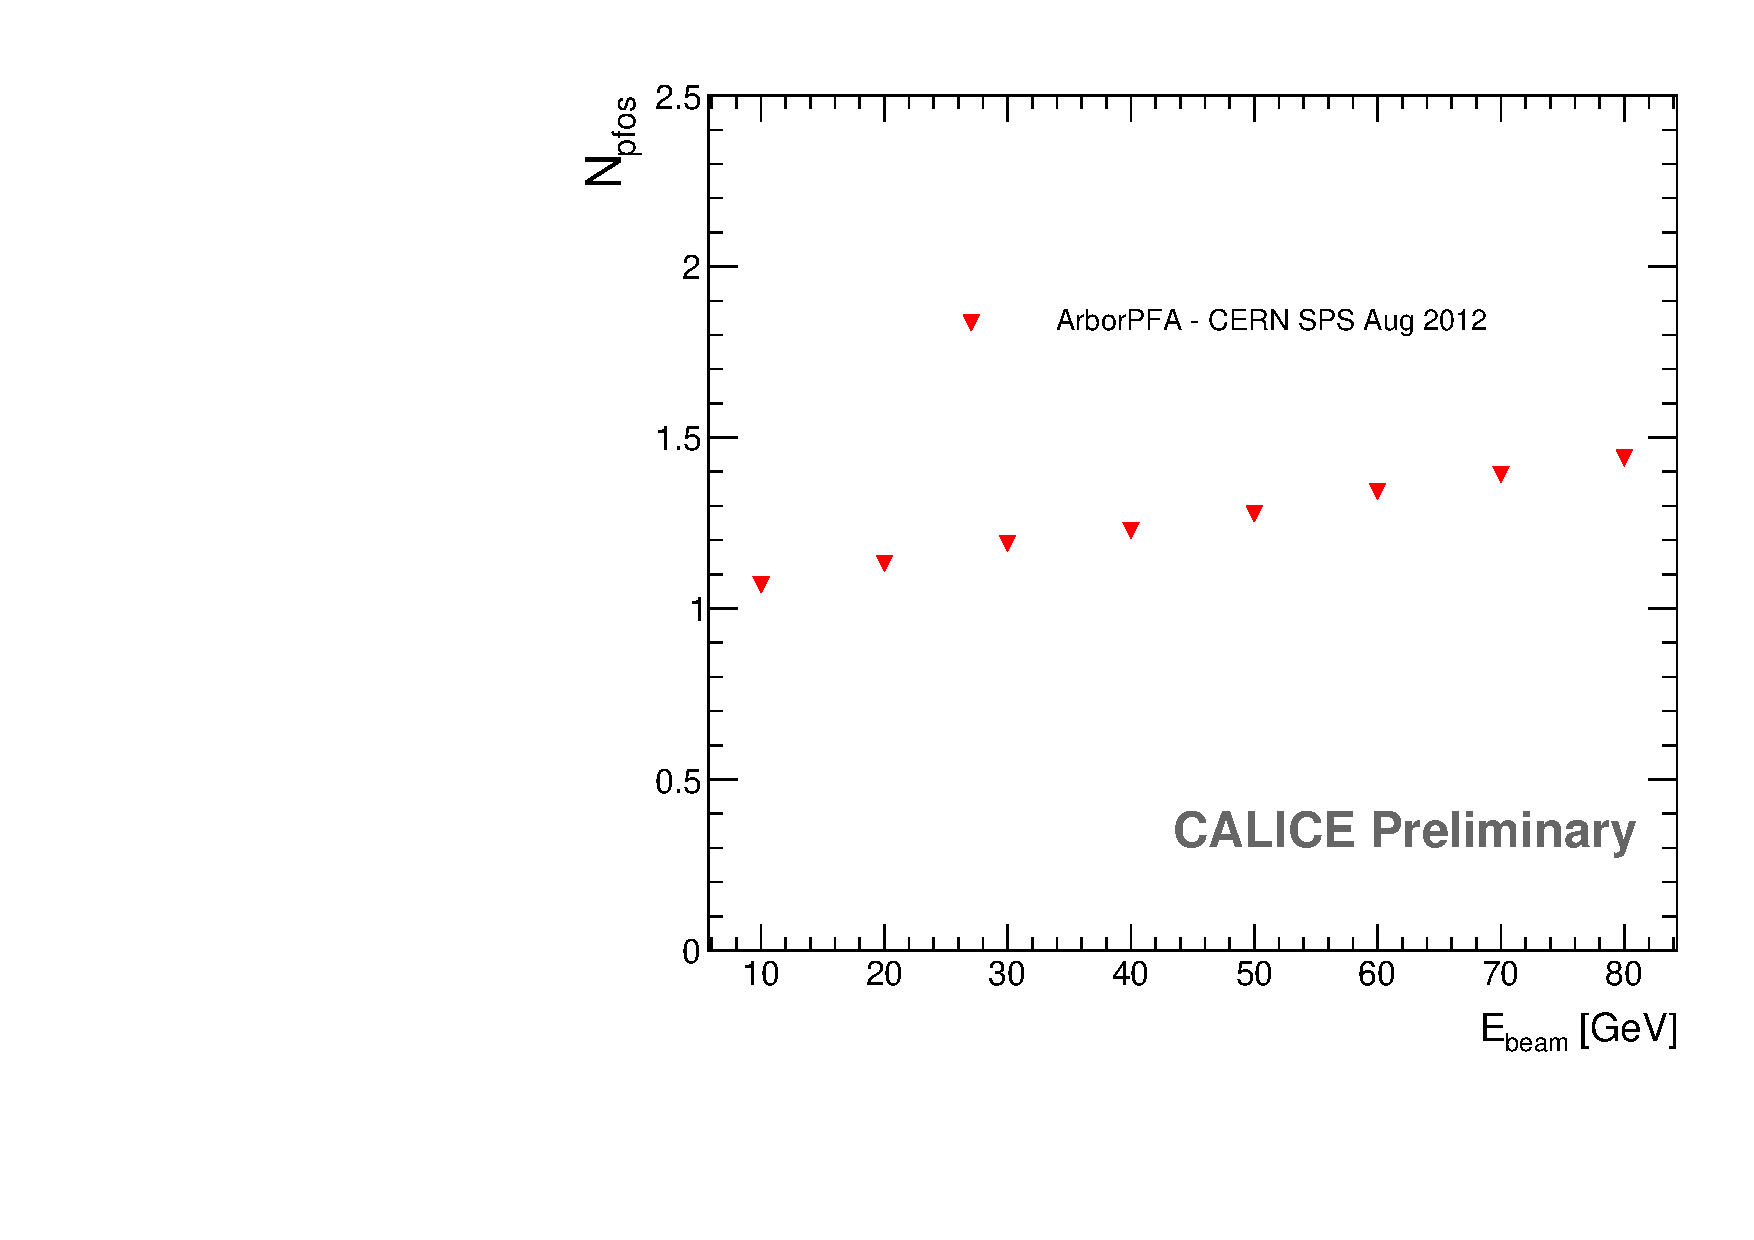
\includegraphics[width=0.5\textwidth]{plots/SingleParticle_NPfos.pdf} \\
      Efficiency $\rightarrow$ OK. NPfos $\rightarrow$ Still a bit of splitting but OK.
    \end{center}
  \end{frame}
  
  
  \begin{frame}
  \frametitle{\secname}
  \framesubtitle{Single particle}
    \begin{center}
      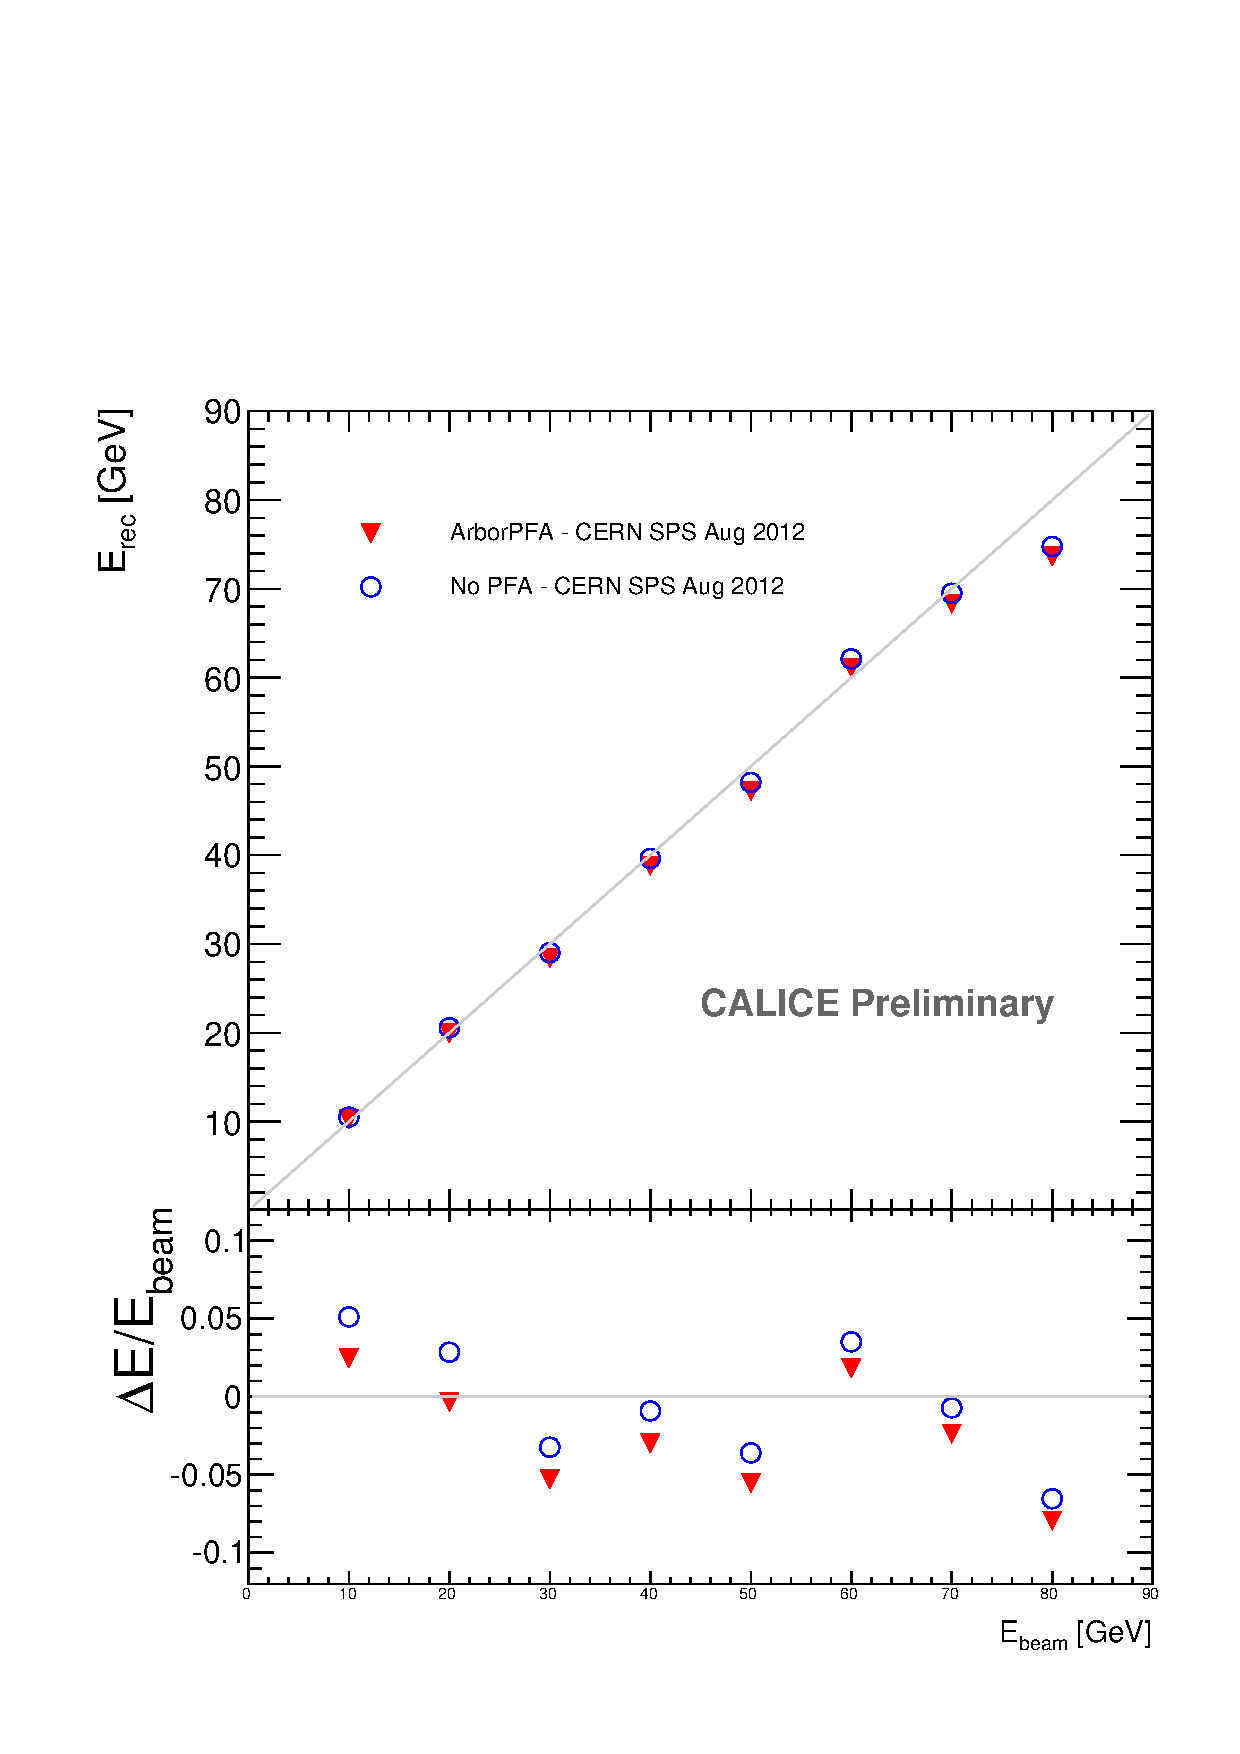
\includegraphics[width=0.5\textwidth]{plots/SingleParticle_ERec.pdf}
      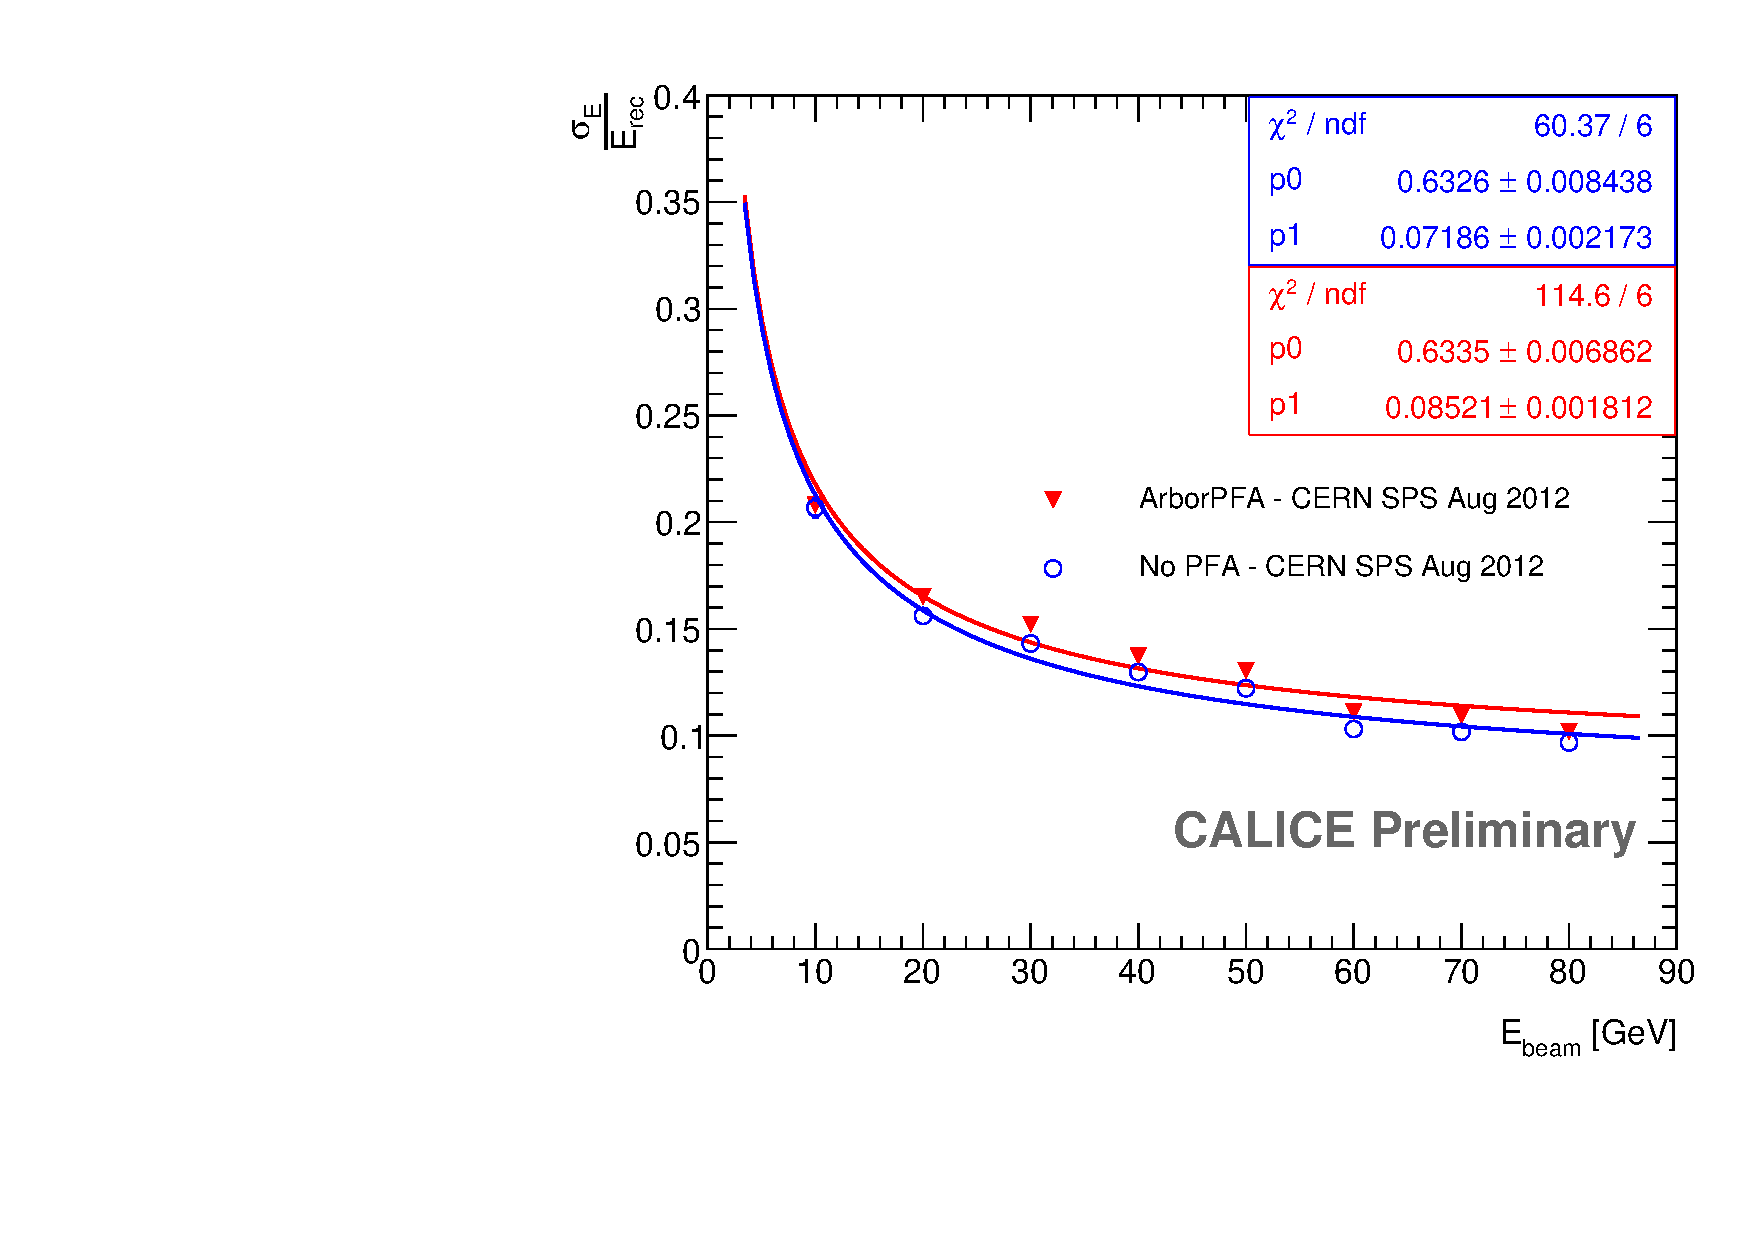
\includegraphics[width=0.5\textwidth]{plots/SingleParticle_EResol.pdf} \\
      ERec $\rightarrow$ Effect of pfo splitting visible in deviation (rather small). \\
      EResol $\rightarrow$ Effect of deviation visible in EResol (Gaussian width remains the same)
    \end{center}    
  \end{frame}
  
  
  \begin{frame}
  \frametitle{\secname}
  \framesubtitle{Overlay events}
    \begin{center}
      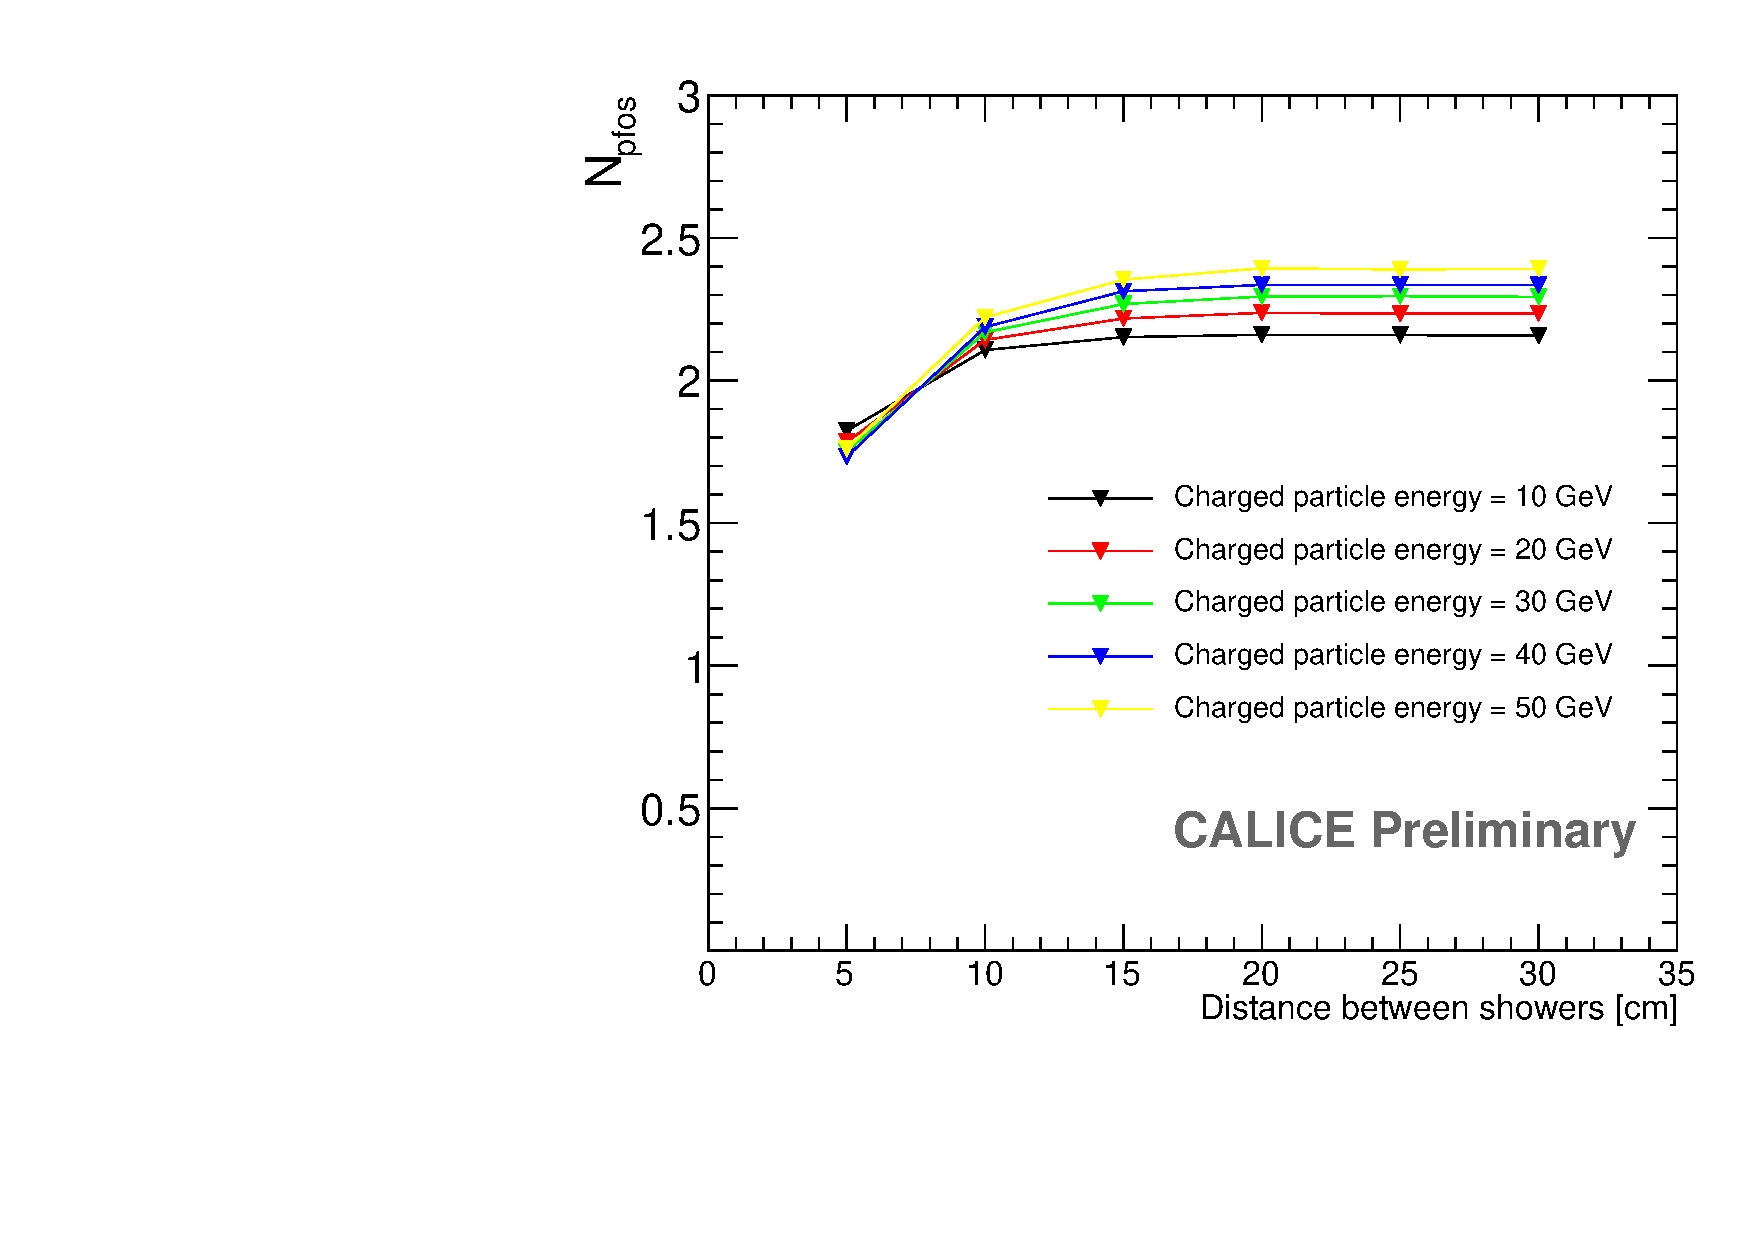
\includegraphics[width=0.5\textwidth]{plots/OverlayEvent_NPfos.pdf} \\
      Compatible with N$_{pfo,n,single}$ + N$_{pfo,ch,single}$ at large distance. \\
      As expected decreasing with the separation distance
    \end{center}
  \end{frame}
  
  
  \begin{frame}
  \frametitle{\secname}
  \framesubtitle{Overlay events}
    \begin{center}
      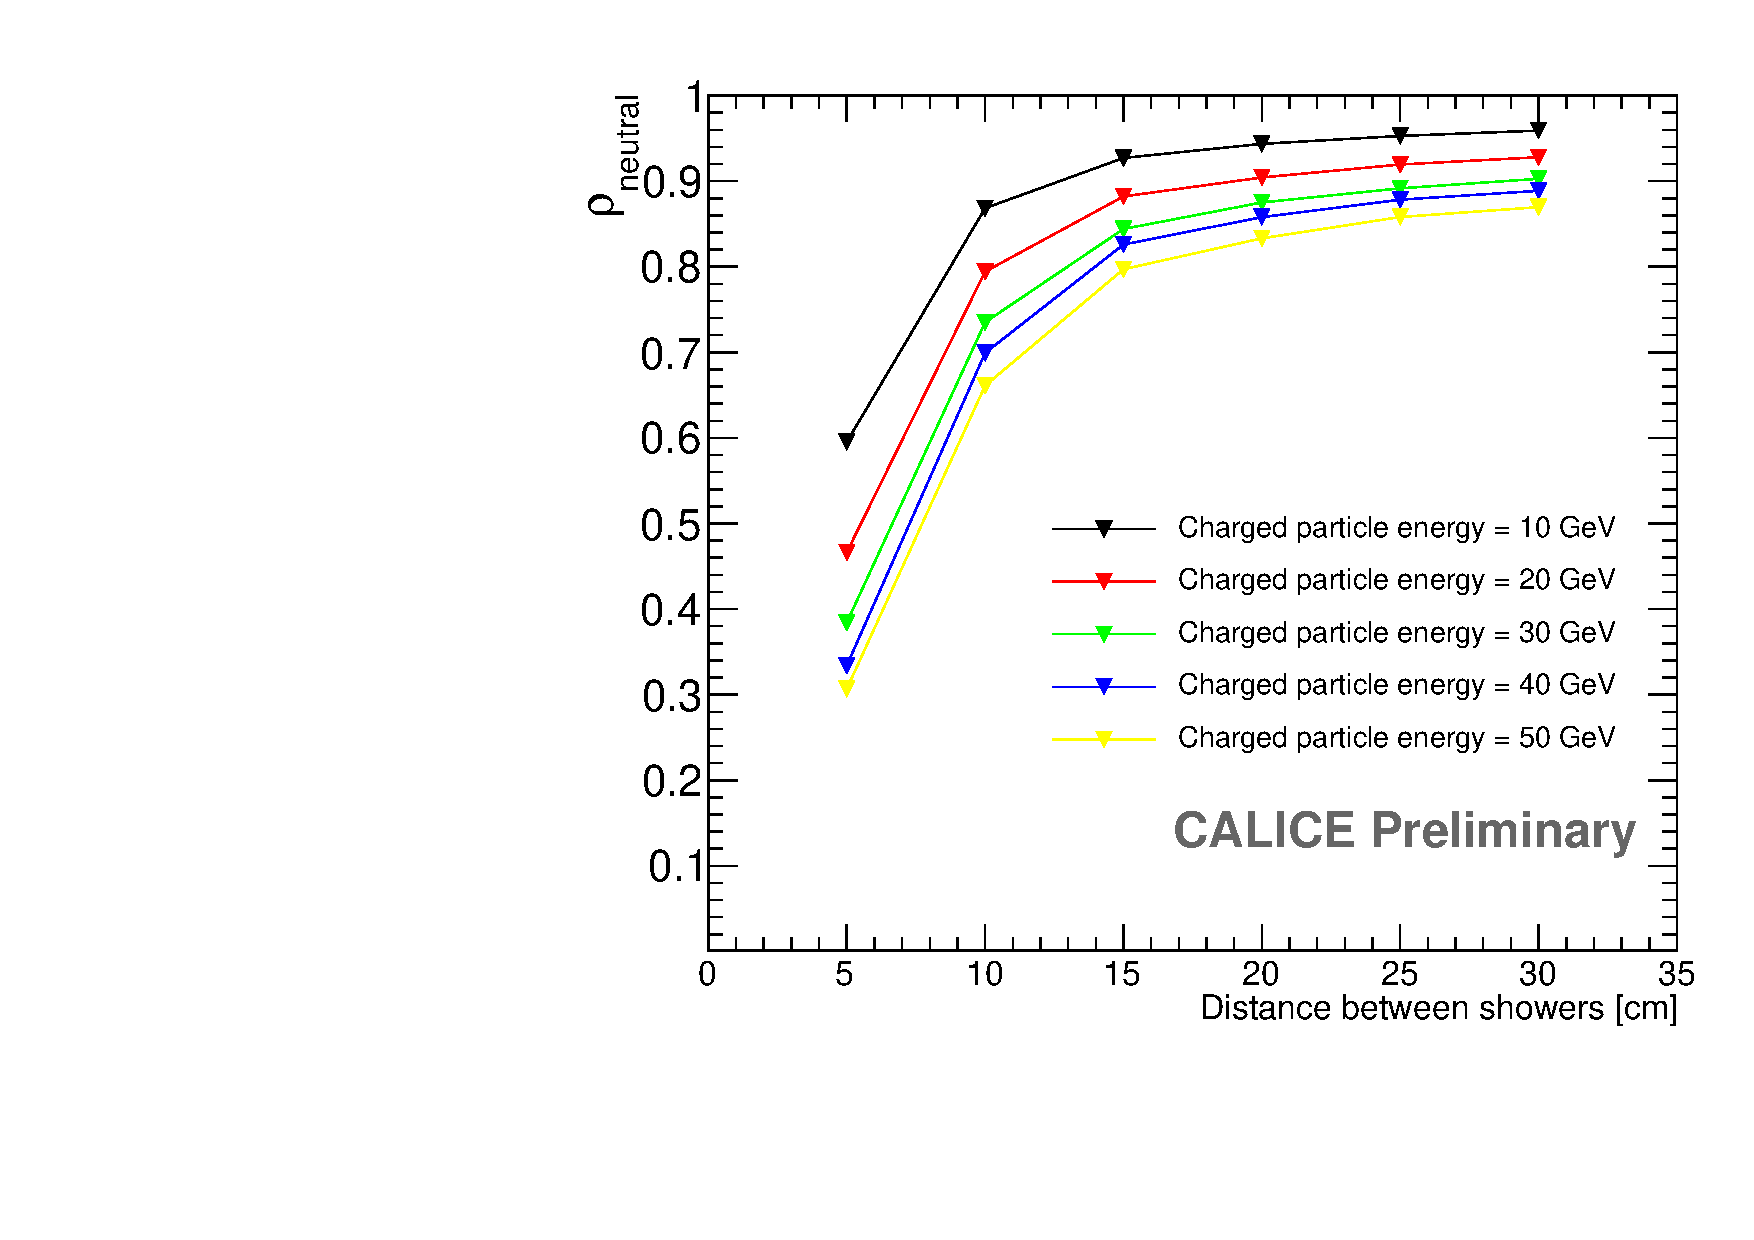
\includegraphics[width=0.5\textwidth]{plots/OverlayEvent_NeutralPurity.pdf}
      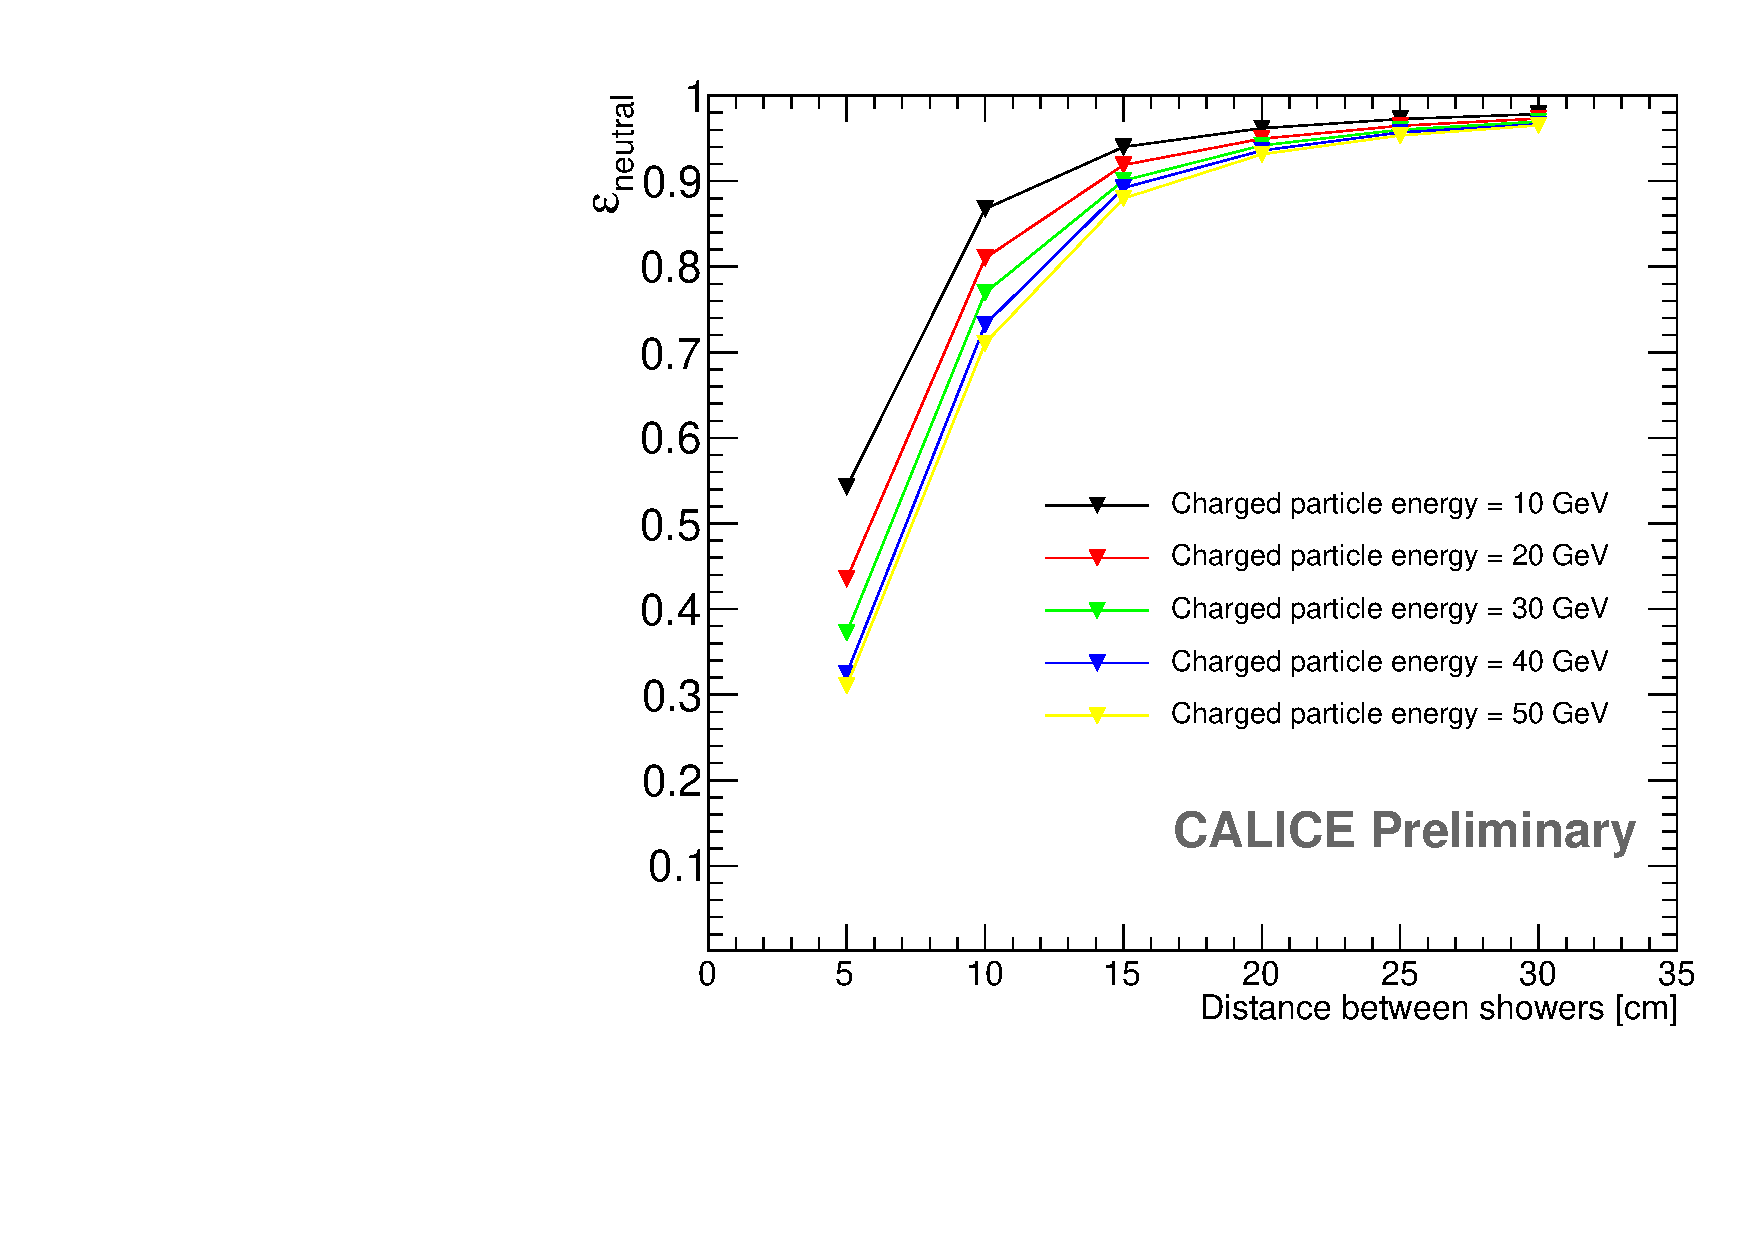
\includegraphics[width=0.5\textwidth]{plots/OverlayEvent_NeutralEfficiency.pdf} \\
      SmallNeutralTreeMerging effect on purity. Using the distance between parent and daughter trees, no energy information (that should be used here !)
    \end{center}
  \end{frame}
  
  \begin{frame}
  \frametitle{\secname}
  \framesubtitle{Overlay events}
    \begin{center}
      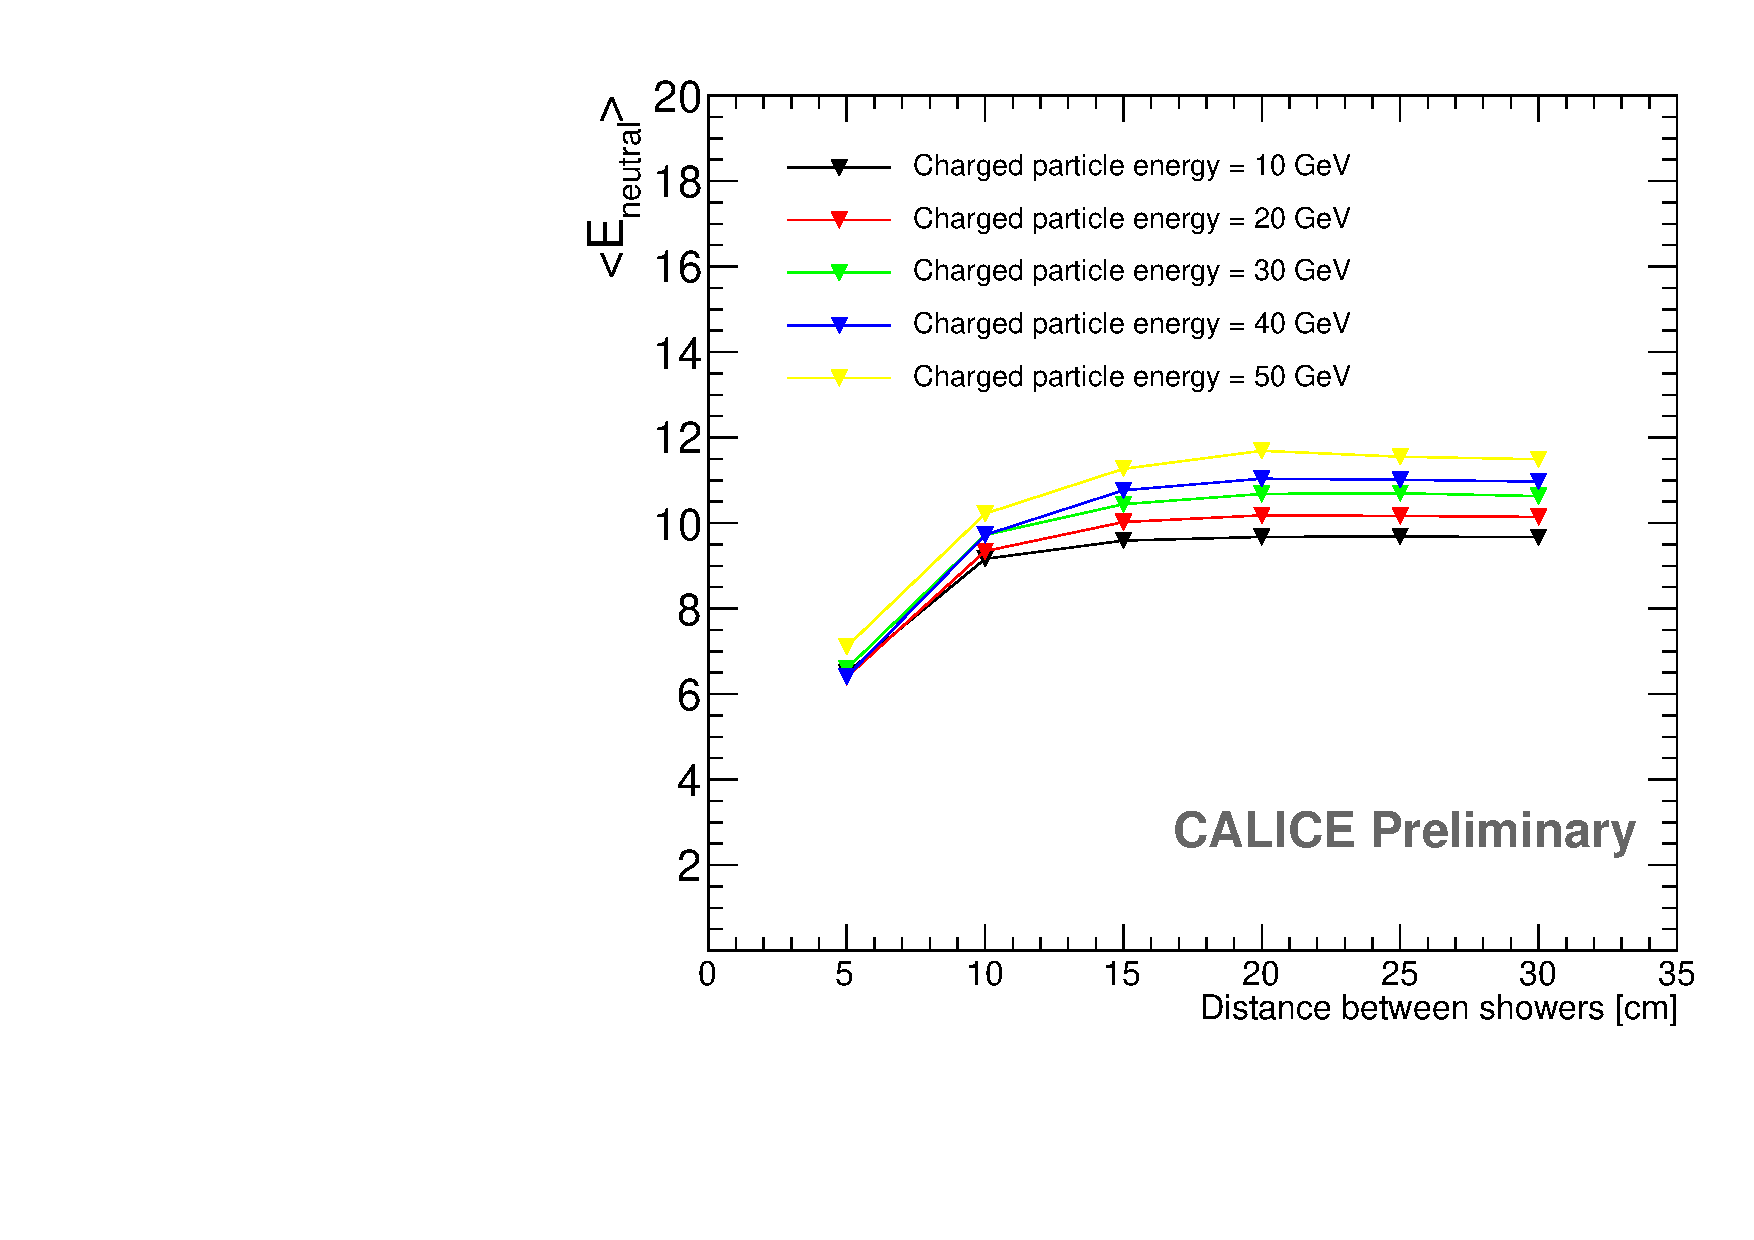
\includegraphics[width=0.5\textwidth]{plots/OverlayEvent_NeutralEnergyMean.pdf}
      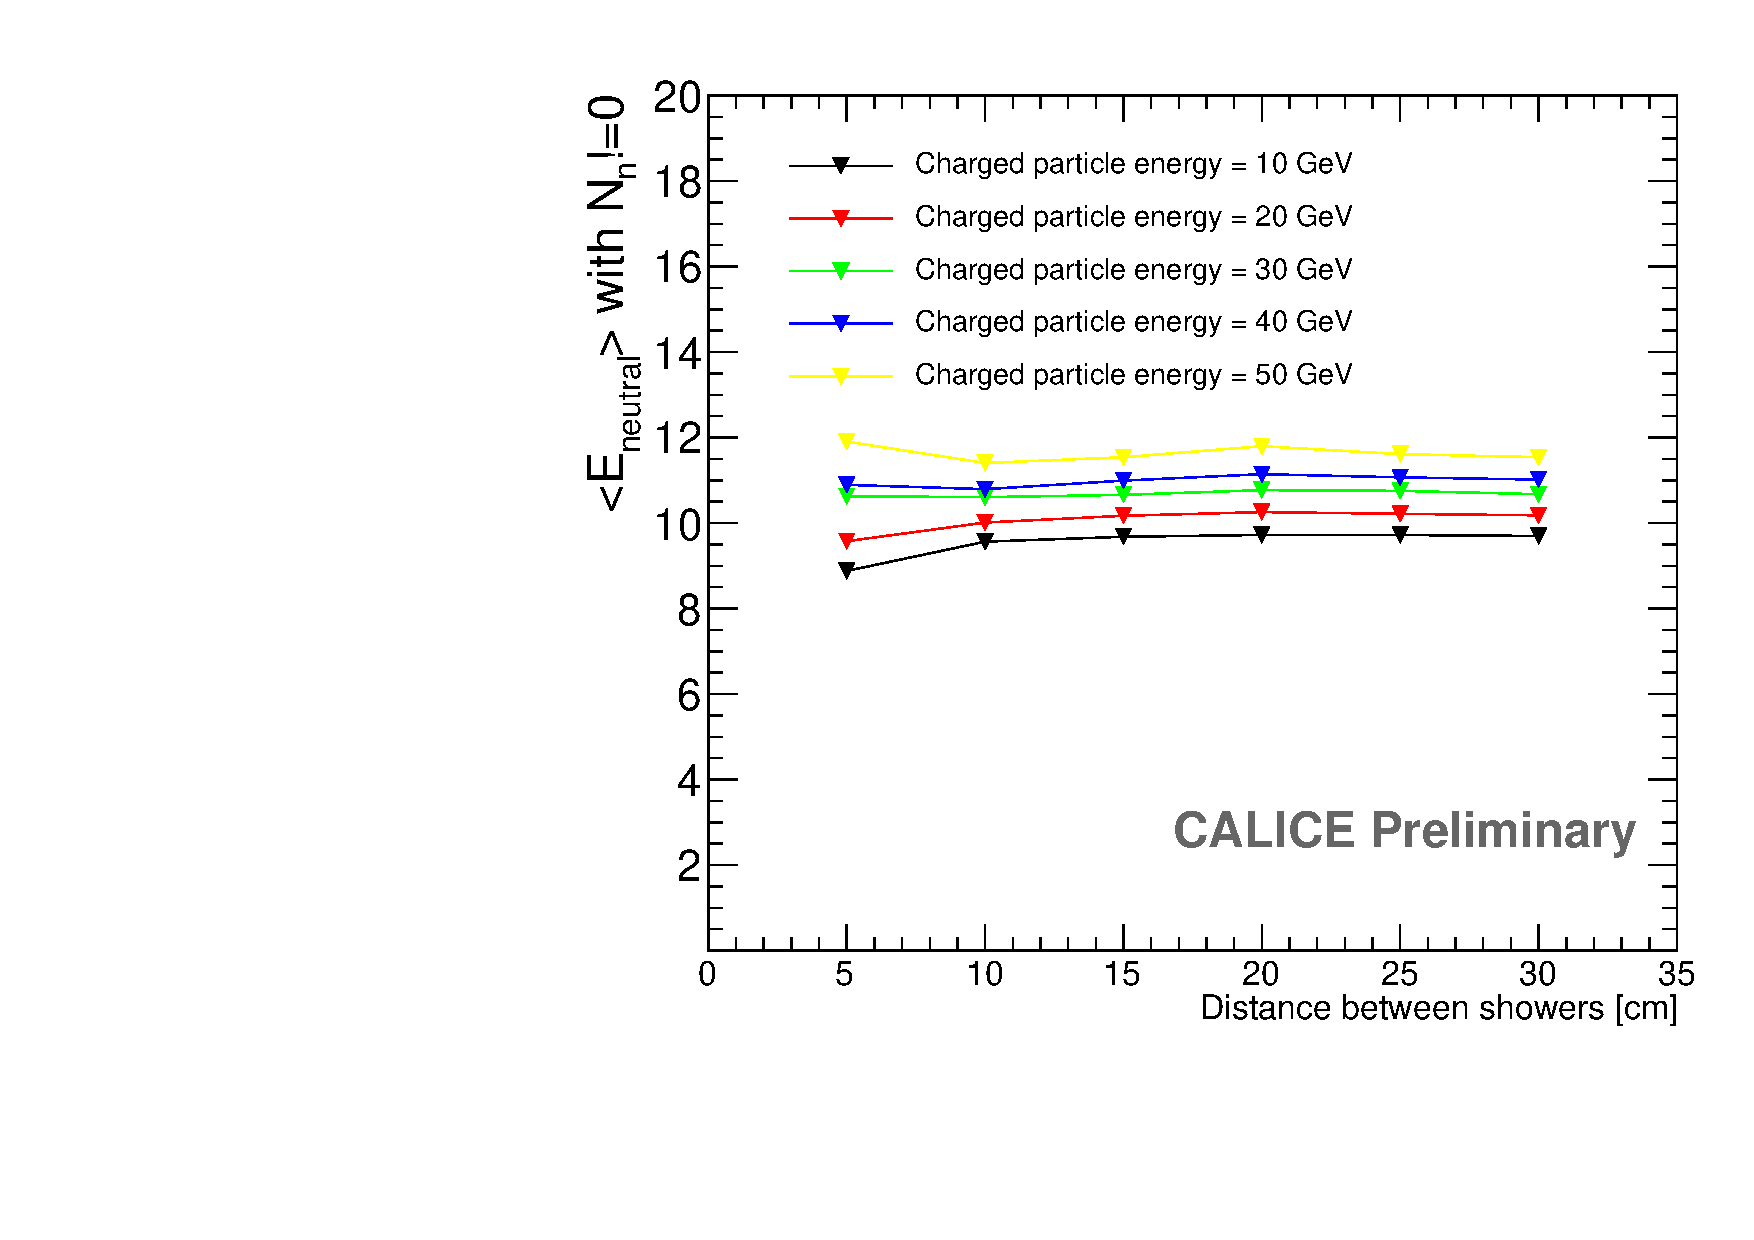
\includegraphics[width=0.5\textwidth]{plots/OverlayEvent_NeutralEnergyMeanNeutralEfficient.pdf} \\
      \begin{itemize}
        \item Again the effect of the SmallNeutralTreeMerging can be seen
        \item Binary-like behavior at small separation distances : good separation or complete merging (event topology)
      \end{itemize}

    \end{center}
  \end{frame}
  
  \begin{frame}
  \frametitle{\secname}
  \framesubtitle{Overlay events}
    \begin{center}
      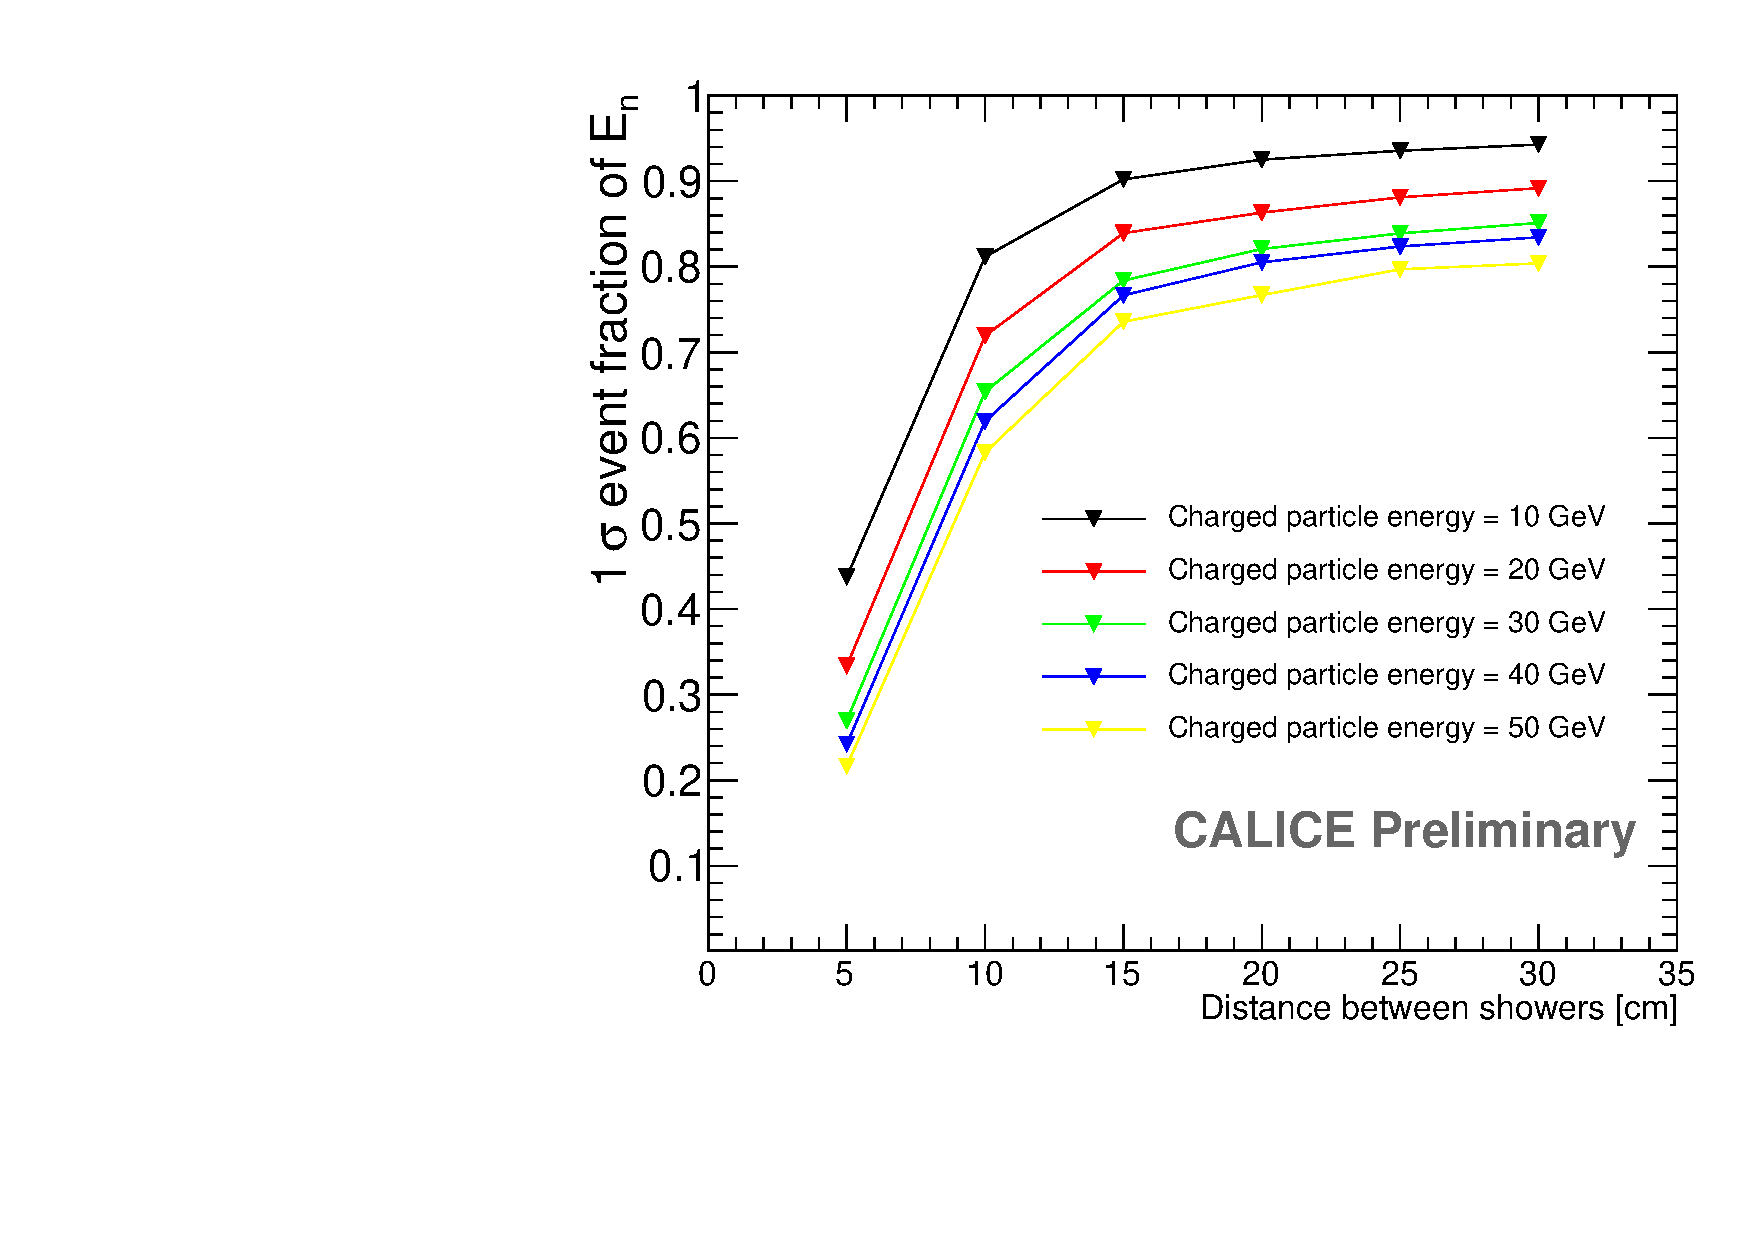
\includegraphics[width=0.5\textwidth]{plots/OverlayEvent_NeutralProba1Sigma.pdf}
      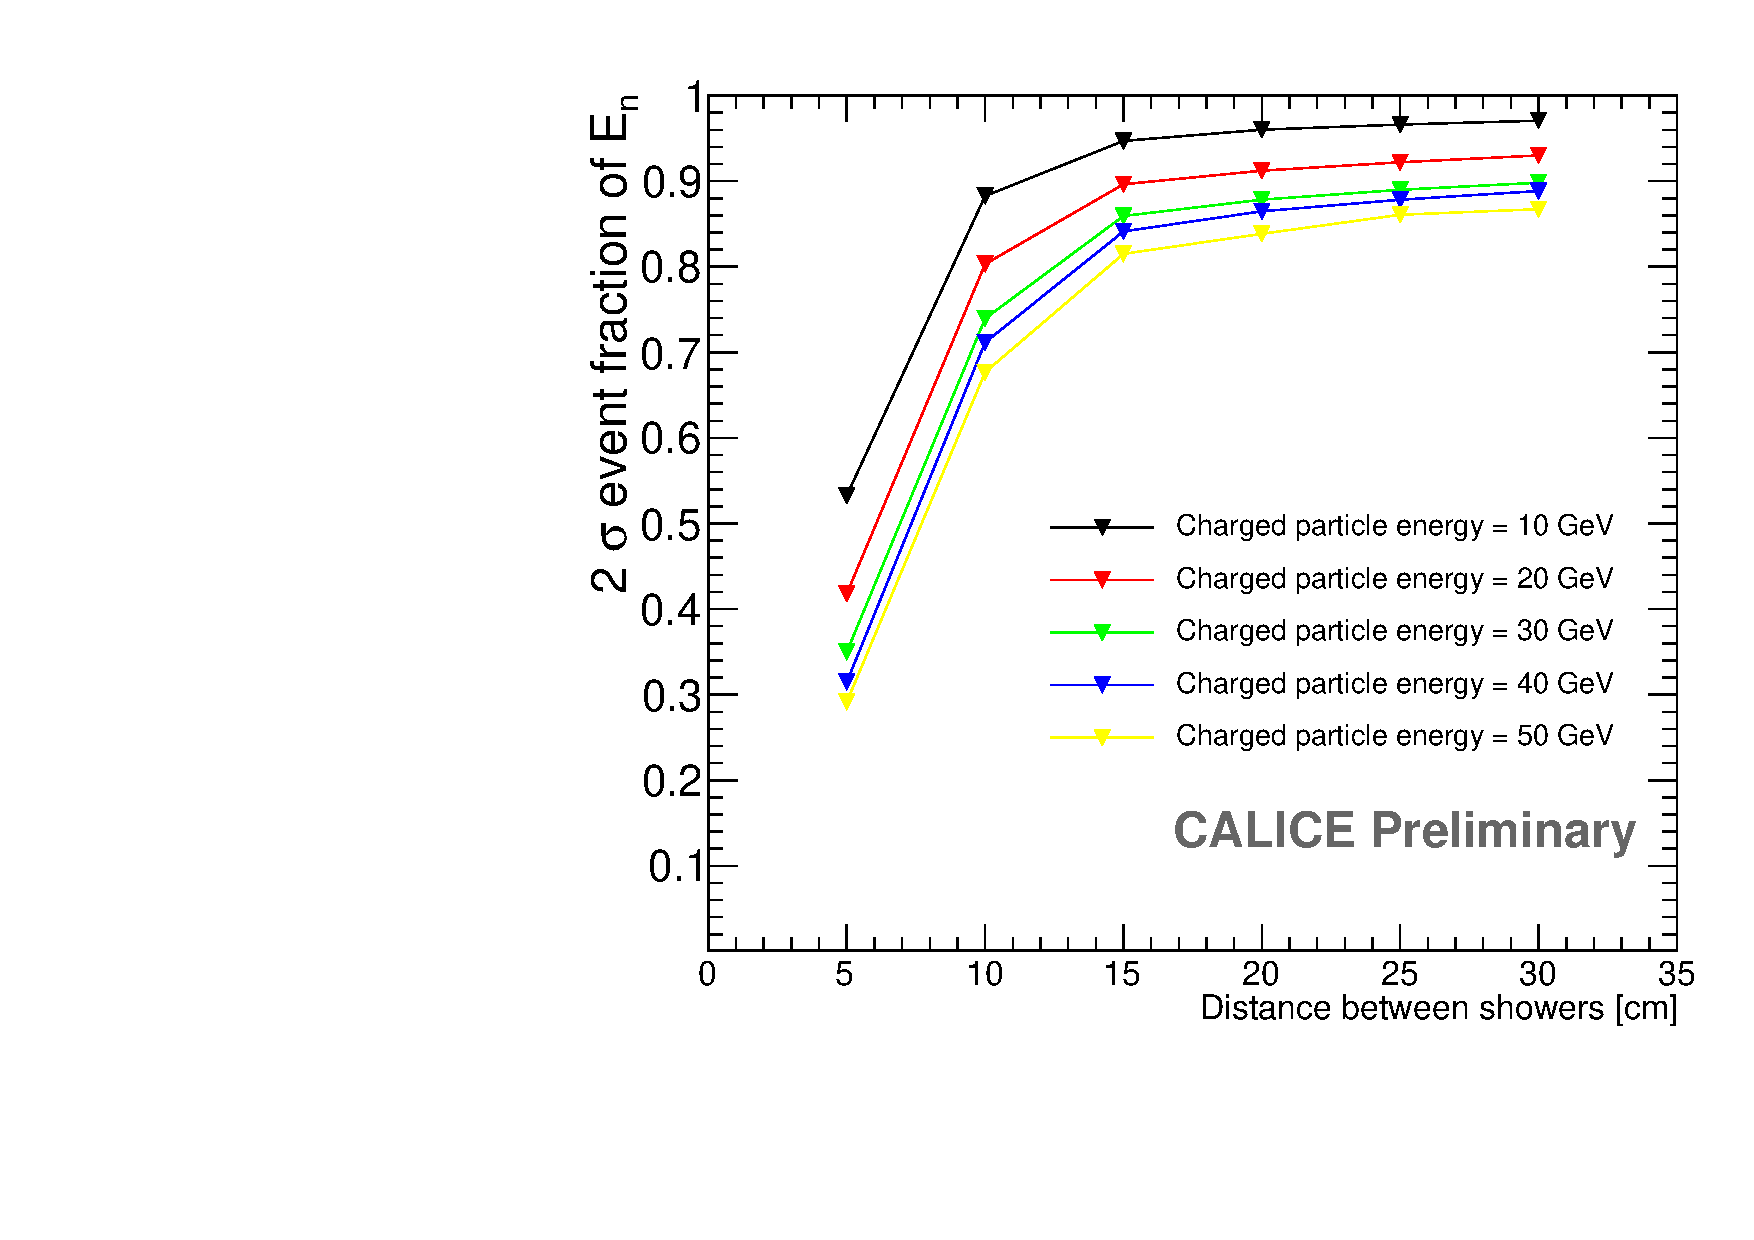
\includegraphics[width=0.5\textwidth]{plots/OverlayEvent_NeutralProba2Sigma.pdf} \\
      Effect of PFA (confusion) + detector (energy resolution)
    \end{center}
  \end{frame}
  
  \begin{frame}
  \frametitle{\secname}
  \framesubtitle{Overlay events}
    \begin{center}
      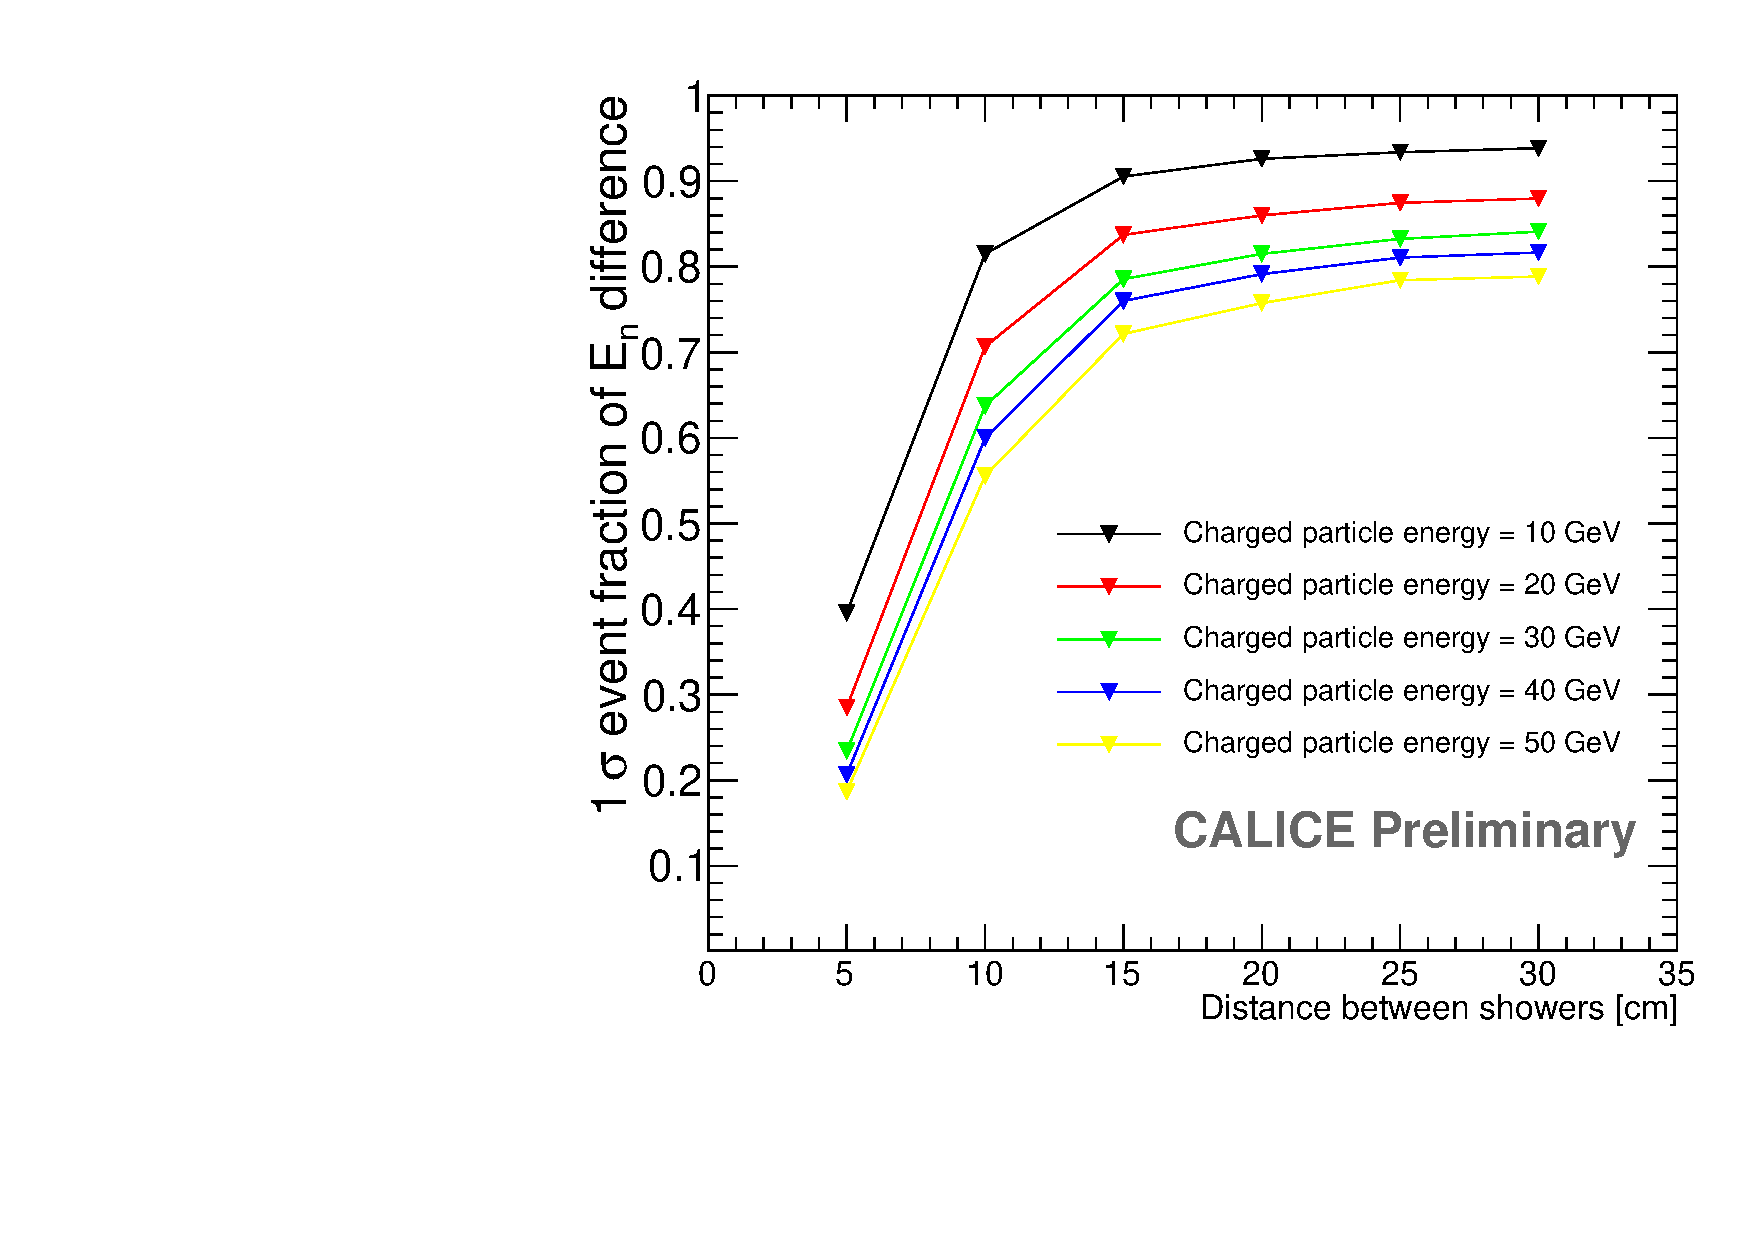
\includegraphics[width=0.5\textwidth]{plots/OverlayEvent_NeutralDifferenceProba1Sigma.pdf}
      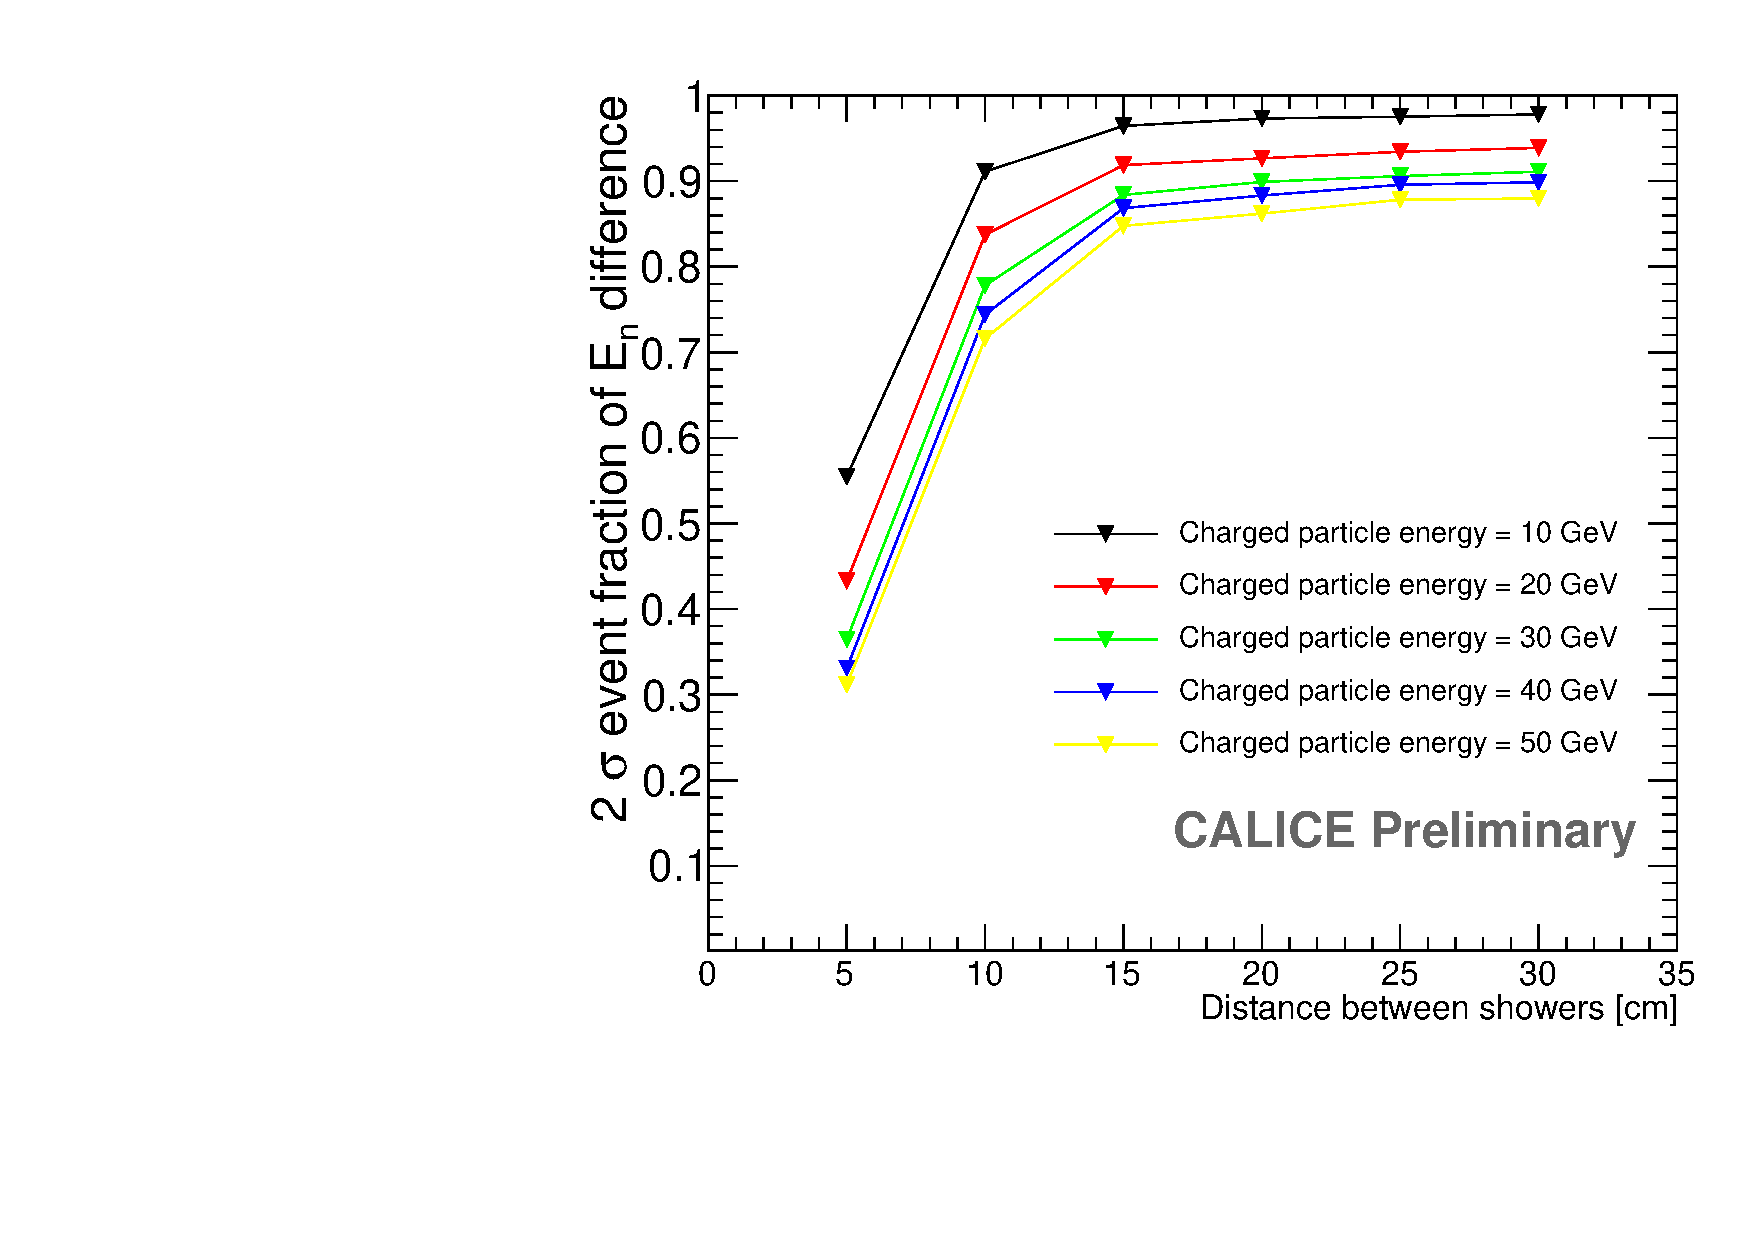
\includegraphics[width=0.5\textwidth]{plots/OverlayEvent_NeutralDifferenceProba2Sigma.pdf} \\
      Effect of PFA only (confusion)
    \end{center}
  \end{frame}
  
  
  \section{Conclusion and forseen work}
  
  \begin{frame}
  \frametitle{\secname}
  
    \begin{block}{Conclusion}
      \begin{itemize}
        \item Single particle understood and shown very good result
        \item Overlaid particle separation understood and shown good results untill 5 cm. At this distance the separation power is binary-like (weel separated or completely merged). Need improvment again ...
      \end{itemize}
    \end{block}
    
    \begin{block}{Current and forseen work}
      \begin{itemize}
        \item Currently working on PandoraSDK development with J. Marshall to make the framework extensible (CaloHit -> ArborCaloHit). This will also make ArborPFA fully compatible with PandoraSDK functionnalities (reclustering, cluster fragmentation).
        \item Finalize the note on the single particle / hadron separation
        \item Correct the isolated tree merging to take into account the main "tree" energy
        \item Finish to rewrite the algorithms in the new SDK framework (almost done)
        \item Implements a reclustering :
        \begin{itemize}
          \item Statistical loop (a la Pandora)
          \item Branch cutting and switching (a la Arbor)
        \end{itemize} 
        \item Starting to look ILD model (ILD\_02\_v05) :
        \begin{itemize}
          \item Implementation in ECal for hadronic interactions
          \item Connection between ECal-HCal
        \end{itemize}
          \item Garlic in ECal and ArborPFA in ECal+HCal looks promising
          \item Start thinking about combined ECal+SDHCAL energy estimator functions
      \end{itemize}
    \end{block}
    
  \end{frame}

\end{document}
